\documentclass[12pt, answers]{exam}
\usepackage{tikz}
\usepackage{amsmath}
\usepackage{amsfonts}
\usepackage{algpseudocodex}
\usepackage{algorithm}
\usepackage{amssymb}
\usepackage{graphicx}
\usepackage{multirow}
\usepackage{enumitem}
\usepackage{subfiles}
\usepackage[most]{tcolorbox} 
\usepackage{changepage} % for adjustwidth
\usepackage{xepersian}

\settextfont[
    Path = ../fonts/,
    Scale = 1.0,
    BoldFont = *Bd,
    ItalicFont = *It,
    BoldItalicFont = *BdIt,
    Extension = .ttf
]{XB Yas}

\renewenvironment{solution}{%
  \par
  \begin{tcolorbox}[
    breakable,                
    colback=white,
    colframe=black,
    arc=1pt,
    boxrule=0.6pt,
    left=4mm, right=4mm,
    top=2mm, bottom=2mm,
    before skip=10pt,
    after skip=10pt,
    segmentation style={solid, black}, 
    before upper={\noindent\textbf{\color{blue}پاسخ:}\par\vspace{0.5em}}
  ]
 }
{%
  \end{tcolorbox}
  \vspace{1em}
}


\algrenewcommand{\algorithmicrequire}{\textbf{Input:}}
\algrenewcommand{\algorithmicensure}{\textbf{Output:}}

\definecolor{codegreen}{rgb}{0,0.6,0}
\definecolor{codegray}{rgb}{0.5,0.5,0.5}
\definecolor{codepurple}{rgb}{0.58,0,0.82}
\definecolor{backcolour}{rgb}{0.95,0.95,0.92}

\lstdefinestyle{mystyle}{
    backgroundcolor=\color{backcolour},   
    commentstyle=\color{codegreen},
    keywordstyle=\color{magenta},
    numberstyle=\tiny\color{codegray},
    stringstyle=\color{codepurple},
    basicstyle=\ttfamily\footnotesize,
    breakatwhitespace=false,         
    breaklines=true,                 
    captionpos=b,                    
    keepspaces=true,                 
    numbers=left,                    
    numbersep=5pt,                  
    showspaces=false,                
    showstringspaces=false,
    showtabs=false,                  
    tabsize=2
}

\lstset{style=mystyle}

% Wide solution environment (extends into the question label area)
% Usage: replace \begin{solution} ... \end{solution} with \begin{widesolution} ... \end{widesolution}
% Keeps the same optional title argument as exam's solution: \begin{widesolution}[عنوان]
\newenvironment{widesolution}[1][]{%
    \begin{solution}[#1]%
    % Outdent left by the current list left margin so the solution spans full text width
    \begin{adjustwidth}{\dimexpr-\leftmargin\relax}{0pt}%
}{%
    \end{adjustwidth}%
    \end{solution}%
}

\renewcommand{\solutiontitle}{\noindent\textbf{\color{blue}پاسخ:}\par}
\newcommand{\class}{داده‌کاوی پزشکی - پایانترم}
\newcommand{\term}{نیم‌سال دوم ۰۴-۰۵}
\newcommand{\college}{دانشکده ریاضی و آمار}
\newcommand{\prof}{جناب آقای دکتر مراتب}
\newcommand{\group}{داوود نصرتی امیرآبادی}

\begin{document}
%%%%%%%%%%%%%% HDR START 
\pagestyle{head}
\firstpageheader{}{}{}
\runningheader{صفحه \thepage\ از \numpages}{}{\class}
\runningheadrule
\begin{tabular}{p{.7\textwidth} l}
    \multicolumn{2}{c}{\textbf{به نام خدا}}                                            \\
                    & \multirow{2}{*}{
\includegraphics[scale=0.2]{../assets/ui-logo.png}} \\
    \textbf{\class} &                                                                  \\
    \textbf{\term}  &                                                                  \\
    \textbf{\prof}  &                                                                  \\
    \textbf{\group} &                                                                  \\
                    & \textbf{\college}
    \\
    % & \textbf{\todaydate} \\
    % & \textbf{\deadline} \\ \\
\end{tabular}\\
\rule[1ex]{\textwidth}{.1pt}

\begin{center}
    \textbf{\lr{امتحان پایان‌ترم}}
\end{center}
%%%%%%%%%%%%%% HDR END 


\begin{questions}
    \pointpoints{نمره}{نمره}
    %%%%%%%%% AZ - 1
    \question سوال ۱:

    \begin{solution}
        داده‌های مسئله عبارتند از:
        $$Se = 0.80, \quad Sp = 0.95, \quad Prev = P(D) = 0.10$$
        در اینجا دیابت داشتن را $D$ در نظر می‌گیریم.

        چیزی که صورت سوال از ما می‌خواهد «احتمال عدم بیماری به شرط مثبت بودن آزمون»
        است. این یعنی
        $P(\bar{D} | T^+)$
        که در اینجا مثبت شدن آزمون را با
        $T^+$
        نشان داده‌ایم.

        با توجه به فرمول‌های بیزی احتمالا شرطی داریم:
        \begin{align*}
            P(A | B)                     & = \frac{P(B | A) P(A)}{P(B)}                 \\
            \Rightarrow P(\bar{D} | T^+) & = \frac{P(T^+ | \bar{D}) P(\bar{D})}{P(T^+)}
        \end{align*}
        خب. در صورت کسر چه داریم؟
        $P(T^+|\bar{D})$.
        این یعنی: احتمال اینکه طرف دیابت نداشته باشد ولی تست ما بگوید او دیابت دارد.
        این همان نرخ مثبت کاذب یا $FPR$ یا $False Positive Rate$ است که از طریق زیر به دست می‌آیدک:
        $$FPR = \frac{FP}{FP + TN} = 1 - Sp = 1 - 0.95 = 0.05$$
        از طرفی عامل دیگر صورت کسر یعنی $P(\bar{D})$
        هم برابر است با $1 - P(D) = 1 - 0.10 = 0.90$

        در مخرج نیز شاهد
        $P(T^+)$
        هستیم. یعنی احتمال اینکه تست یکی از کودکان مثبت شود.
        دو حال داریم. یا اینکه این کودک واقعا دیابت دارد و تست  او مثبت شده است. یا اینکه
        دیابت ندارد و تست او مثبت شده است. یعنی:
        $P(D \cap T^+)$
        و
        $P(\bar{D} \cap T^+)$.
        پس در ادامه خواهیم داشت:
        \begin{align*}
            P(D \cap T^+)       & = P(D) \times P(T^+ | D)  = Prev \times Se = 0.10 \times 0.80 = 0.080                   \\
            P(\bar{D} \cap T^+) & = P(\bar{D}) \times P(T^+ | \bar{D}) = (1 - Prev) \times FPR = 0.90 \times 0.05 = 0.045
        \end{align*}
        از طرفی چون این دوحالت هیچ اشتراکی با هم ندارند می‌توانیم آن‌ها را به راحتی با هم جمع کنیم
        تا مقدار مورد نظر در مخرج را به دست آوریم.
        پس خواهیم داشت:
        $$P(\bar{D} | T^+) = \frac{P(T^+ | \bar{D}) P(\bar{D})}{P(T^+)} = \frac{0.05 \times 0.90}{0.080 + 0.045} = \frac{0.045}{0.125} = 0.36 $$
        پس احتمال شرطی عدم بیماری به شرط مثبت بودن آزمون برابر با
        $36\%$
        است. این یعنی از میان کودکانی که نتیجه تست و آزمون دیابت آن‌ها مثبت از آب در می‌آید،
        $36$ درصد واقعا دیابت ندارند و صرفا نتیجه آزمونشان مثبت کاذب بوده است.

        البته بعد از محاسبه پاسخ به این روش متوجه شدم که با استفاده از
        فرمول $FDR$ می‌توان به پاسخ مورد نظر رسید چرا که تعریف
        $FDR$ همان مقدار مورد نظر سوال است.

        داریم:
        \begin{align*}
            FDR             & = \frac{FP}{FP + TP} = 1 - PPV                                            \\
            PPV             & = \frac{Se \times Prev}{(Se \times Prev) + ((1 - Sp) \times (1 - Prev))}  \\
                            & = \frac{0.80 \times 0.10}{(0.80 \times 0.10) + (0.05 \times 0.90)} = 0.64 \\
            \Rightarrow FDR & = 1 - 0.64 = 0.36
        \end{align*}

    \end{solution}

    \pagebreak

    %%%%%% AZ - 2

    \question سوال ۲:

    \begin{solution}
        گرچه در صورت سوال ذکر نشده اما باید دقت داشته باشیم که برای
        استفاده از روشی توکی، لازم است که میزان Skewness
        داده ها مشخص شود که اگر زیاد باشد، توکی به درستی عمل نخواهد کرد. طبق گفته های استاد در کلاس این به دلیل آن است که ضریب ۱.۵ که
        در ادامه به آن اشاره میکنیم با فرض نرمال توزیع داده ها در نظر گرفته شده است
        و در صورت نرمال نبودن توضیح دیگر نمیتوان از این ضریب استفاده کرد.
        $$\text{Pearson Skewness} = \frac{3 \times (mean - median)}{standard\ deviation}$$
        این مقدار را برای داده های موجود در صورت سوال انجام دادیم:
        \begin{center}
            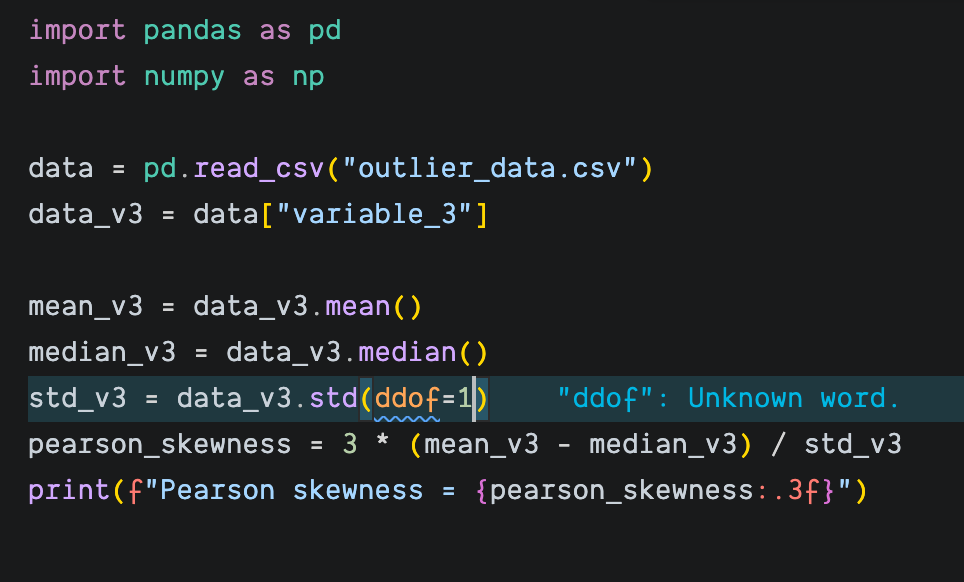
\includegraphics[width=0.65\textwidth]{figures/q2-skewness-code.png}
            
\includegraphics[width=0.65\textwidth]{figures/q2-skewness-result.png}
        \end{center}
        تحلیل جواب به این صورت است که توزیع مورد بحث ما چولگی خاصی به سمت راست و چپ ندارد و داده به طور متوازن پخش شده است.
        درواقع اگر این عدد کمتر از
        $-1$
        میبود میگفتیم که چولگی به سمت چپ است و اگر بیشتر از
        $1$
        میبود میگفتیم چولگی به سمت راست است.

        حالا به سراغ کار با روش توکی می‌رویم. ابتدا چارک اول و سوم را به دست آورده و از هم کم می‌کنیم تا مثدار
        $IQR$ به دست آید.
        سپس چارک اول را منهای
        $1.5$ برابر مقدار $IQR$
        کرده و کران پایین مینامیم. همچنین، چارک سوم را به علاوه‌ی
        $1.5$
        برابر مقدار $IQR$
        کرده و کران بالا می‌نامیم. این ضریب $1.5$ همان ضریبی است که گفتیم بر مبنای نرمال بودن داده‌ها از آن استفاده می‌کنیم.
        در نهایت داده‌های خارج از این کران را داده‌ی پرت در نظر می‌گیریم.

        \begin{center}
            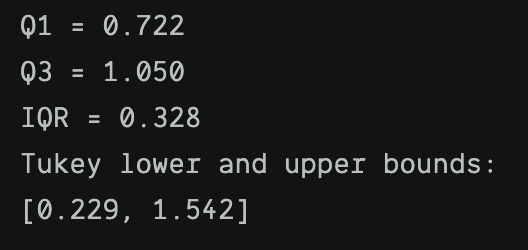
\includegraphics[width=0.32\textwidth]{figures/q2-tukey-result.png}
            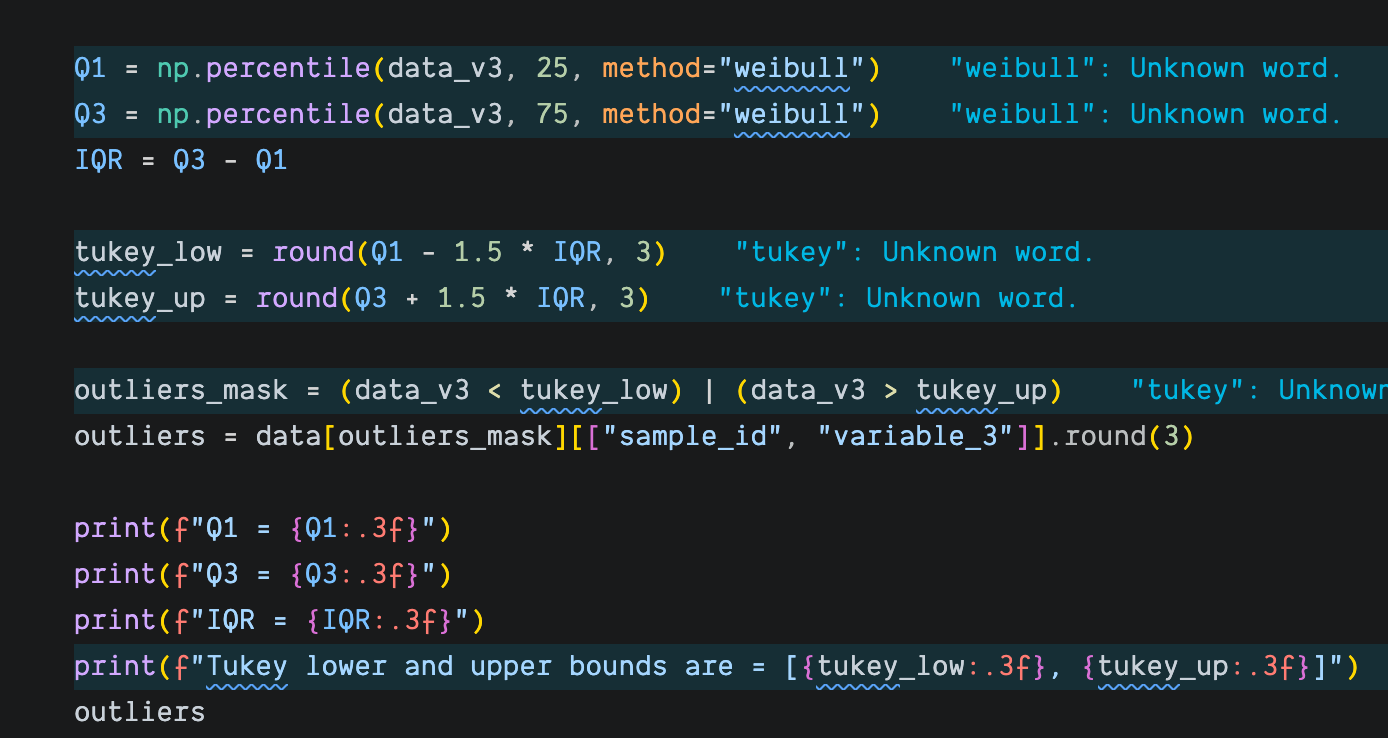
\includegraphics[width=0.65\textwidth]{figures/q2-tukey-code.png}
        \end{center}

        همانطور که مشخص است سمپلهای
        $14, 39, 66, 101$
        داده پرت محسوب شده‌اند.

        در مورد بخش انتهایی سوال هم باید این نکته را را مد نظر داشته باشیم که احتمالهای مختلفی
        اعم از اشتباه ایجنت انسانی وارد کننده اطلاعات، تبدیلات عددی غیرمنتظره در ماشین، نمایش نامناسب اعداد و ... ممکن است باعث ایجاد خطا
        شده و داده را به اشتباه پرت محسوب کنند. پس نباید داده‌ها را طی یک روند اتوماتیک پس از تشخیص پرت بودن حذف کنیم.
    \end{solution}


    \pagebreak
    %%%%%%%%%%%% AZ 3
    \question سوال ۳:

    \begin{solution}
        ابتدا از منوی \lr{File -> Import data -> CSV data} اقدام به وارد کردن داده‌ها میکنیم.
        سپس طبق تصویر به منوی
        \lr{Data -> Select Cases}
        وارد شده و گزینه \lr{If condition is satisfied} را انتخاب میکنیم.
        بعد مطابق خواسته ی سوال، شرط
        \text{$outcome\_cad = 0$}
        را نوشته و تایید میکنیم.
        \begin{center}
            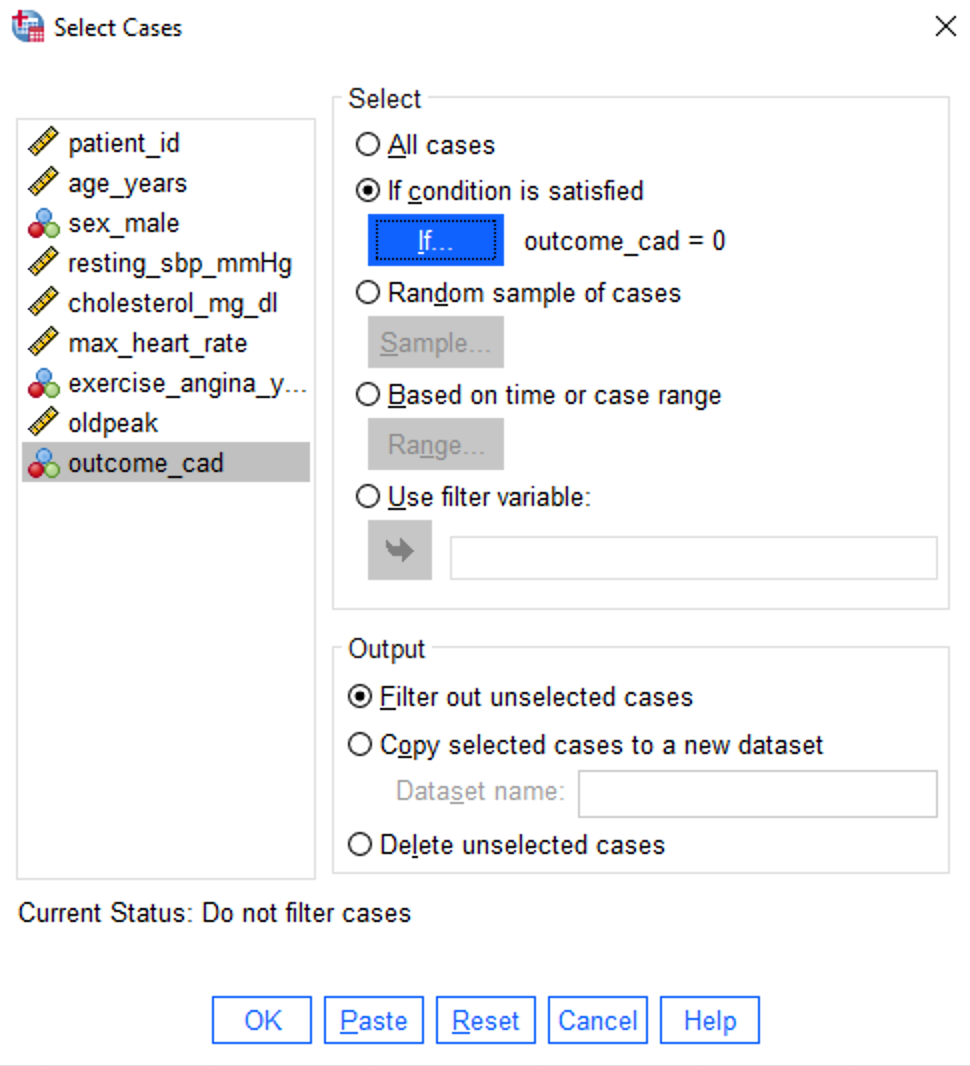
\includegraphics[width=0.65\textwidth]{figures/q3-select-cases.png}
            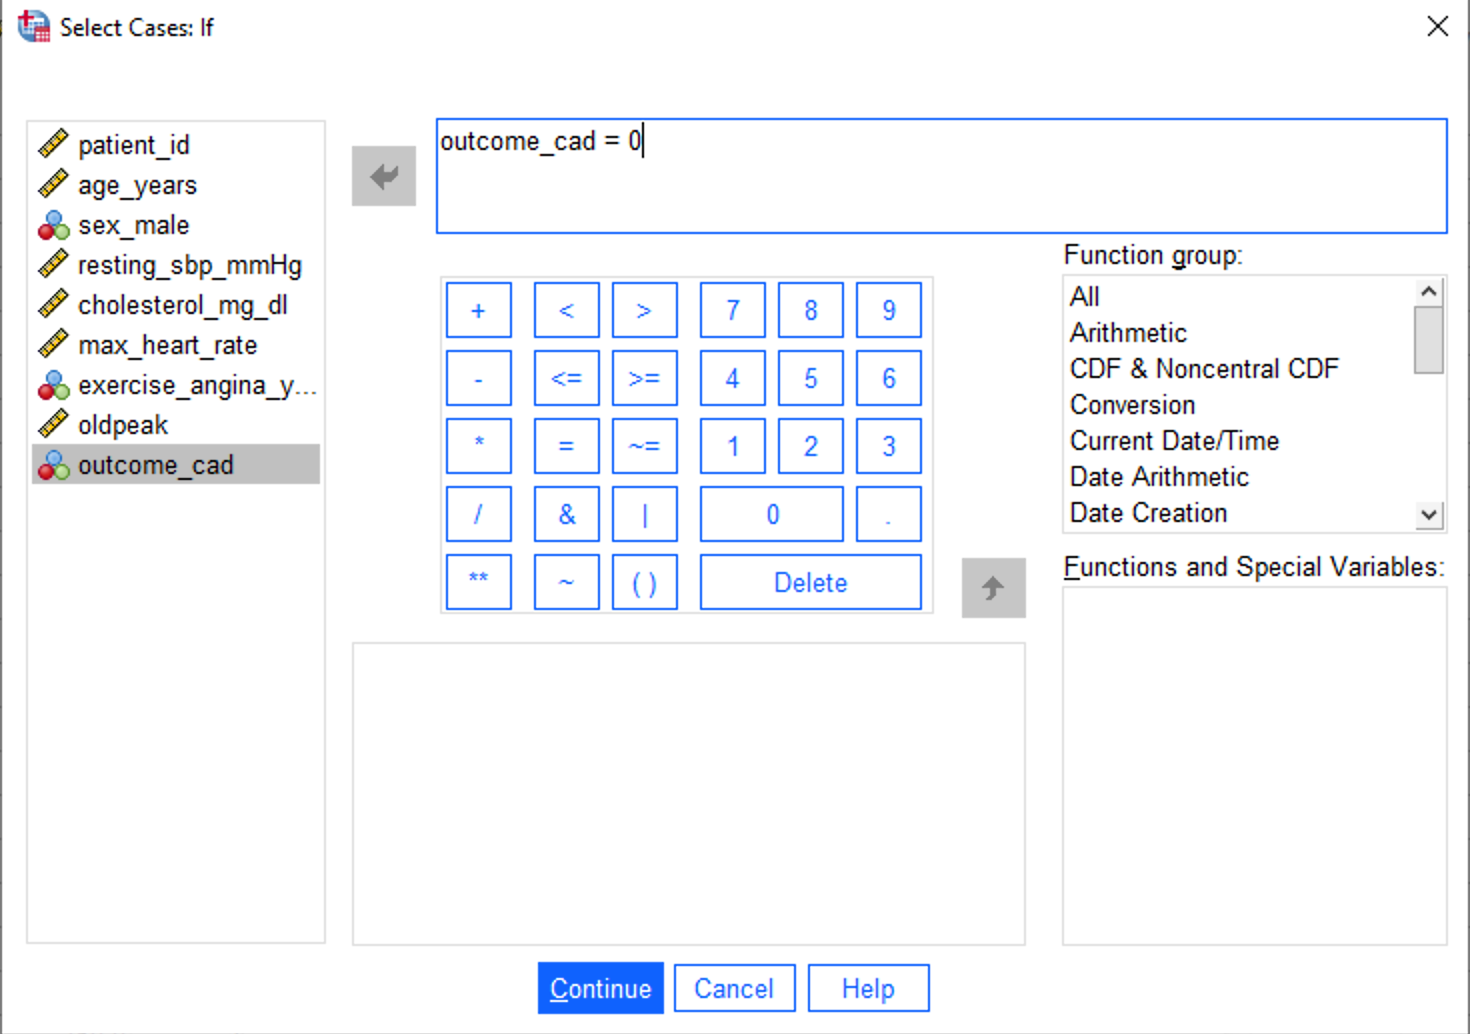
\includegraphics[width=0.65\textwidth]{figures/q3-select-cases-condition.png}
        \end{center}

        به منظور بررسی همبستگی بین متغیرها ابتدا باید نوع آنها را مشخص کنیم.
        وقتی به ستونهای متناظر آنها نگاه کرده و مقادیر را بررسی می‌کنیم
        متوجه میشویم که هر دو از نوع Interval هستند.
        بعد از این، باید نرمال بودن آنها را مورد بررسی قرار دهیم.
        در این جا باید به این نکته دقت کنیم که تعداد داده‌های ما چند تاست.
        با توجه به شرطی که در ابتدا لحاظ کردیم ۱۵۷ داده برای ما باقی مانده است که به ما اجازه استفاده از تست
        کولموگروف-اسمیرنوف را می‌دهد.

        از منوی
        \lr{Analyze -> Nonparametric Tests -> Legacy Dialogs -> 1 Sample K-S}
        وارد شده و متغیرهای مورد نظر را انتخاب میکنیم. سپس در قسمت \lr{Test Distribution} گزینه \lr{Normal} را انتخاب کرده و روی گزینه
        \lr{OK}
        کلیک میکنیم:
        \begin{center}
            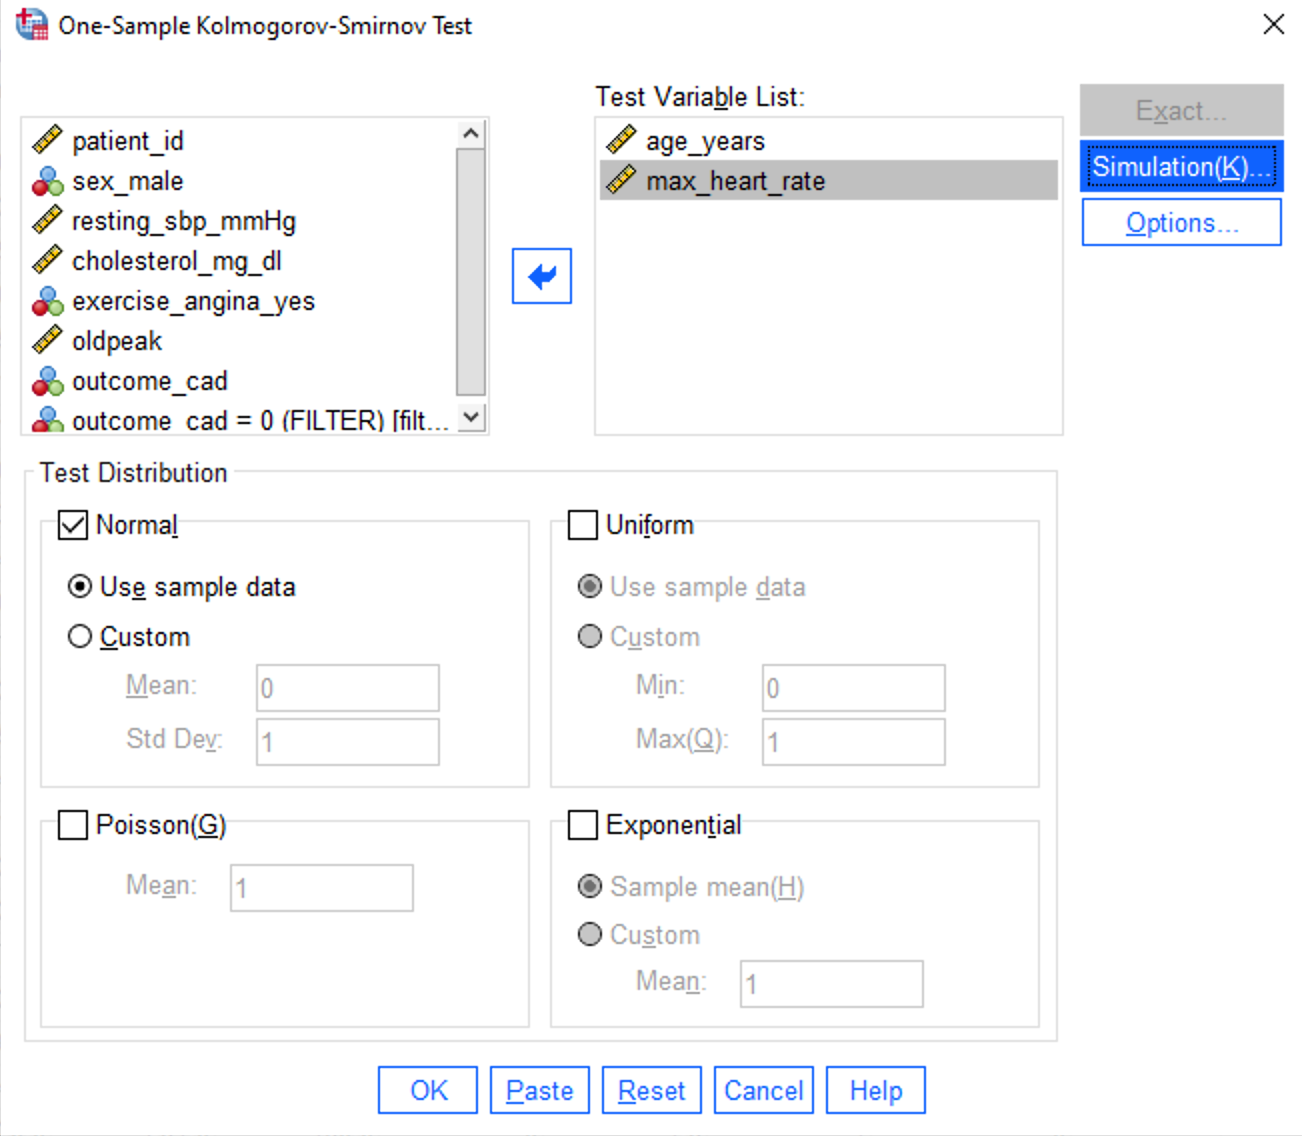
\includegraphics[width=0.65\textwidth]{figures/q3-ks-test-dialog.png}
        \end{center}

        نتایج این تست به صورت زیر است:
        \begin{center}
            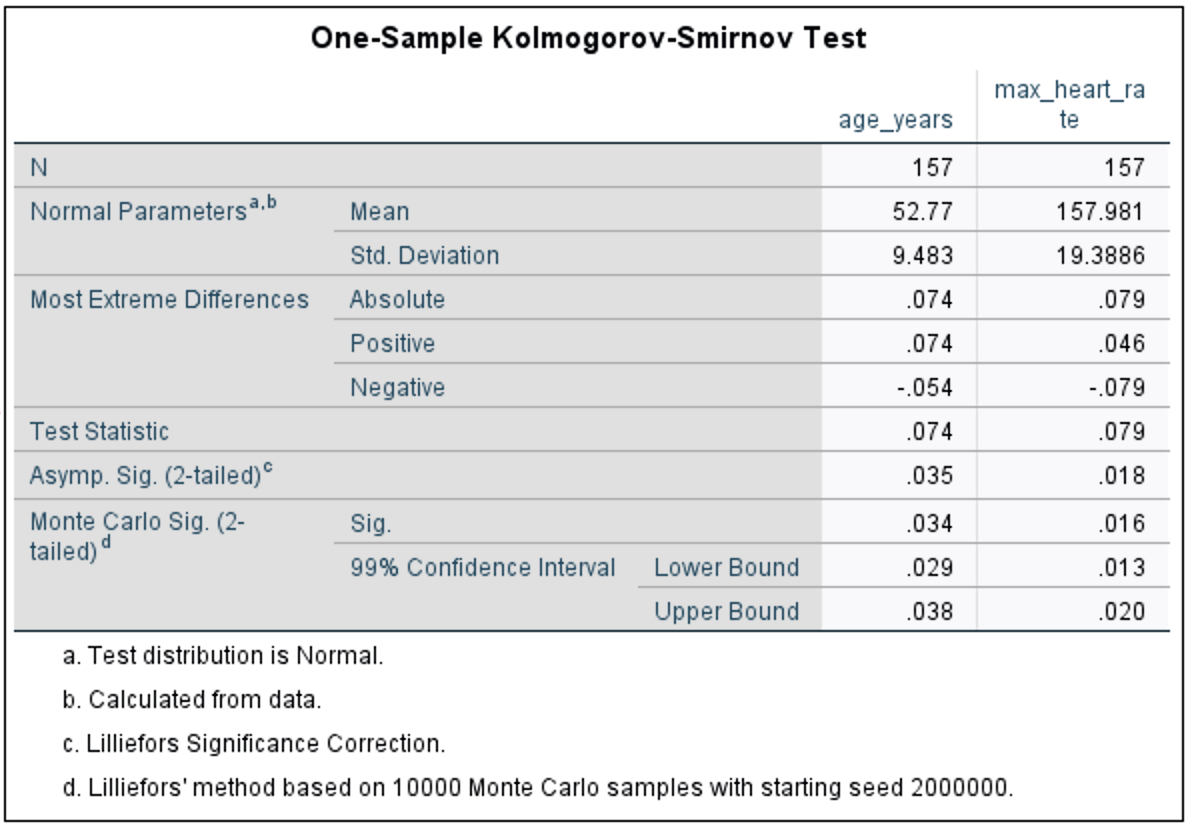
\includegraphics[width=0.65\textwidth]{figures/q3-ks-test-result.png}
        \end{center}
        همانطور که می‌بینم مقدار
        $p-value$
        برای هر دو متغیر
        $age\_years$ و $max\_heart\_rate$
        برابر با
        $0.035$ و $0.016$
        است که هر دو کمتر از
        $0.05$
        هستند و این یعنی از توزیع نرمال پیروی نمی‌کنند.

        در نتیجه با توجه به نتایج باید تست
        $Spearman$
        بگیریم.
        برای این کار از منوی
        \lr{Analyze -> Correlate -> Bivariate}
        وارد شده و متغیرهای مورد نظر را انتخاب میکنیم.
        سپس تیک گزینه \lr{Spearman} را زده و سپس
        تیک گزینه
        \lr{Pearson}
        را برمیداریم
        و روی گزینه
        \lr{OK}
        کلیک میکنیم:
        \begin{center}
            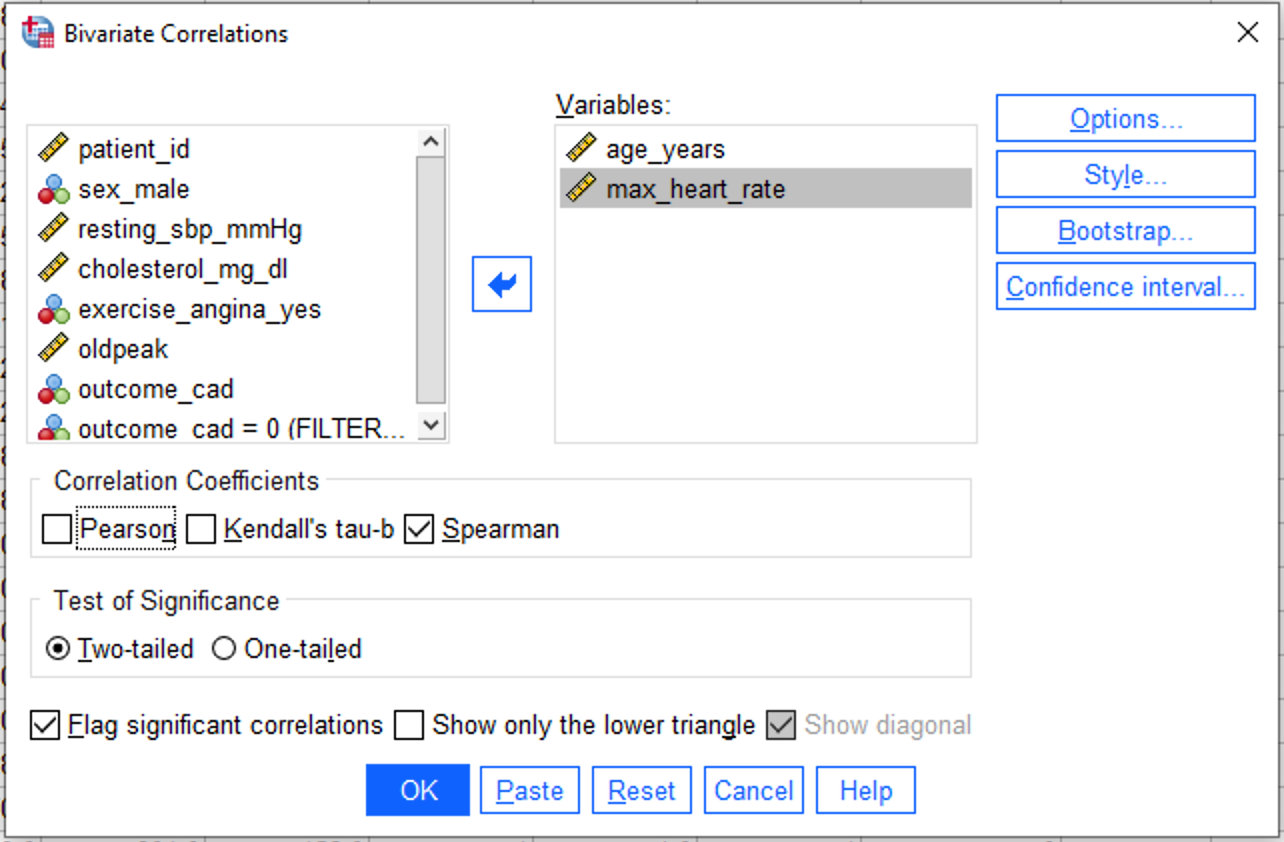
\includegraphics[width=0.65\textwidth]{figures/q3-spearman-dialog.png}
        \end{center}

        نتایج به صورت زیر هستند:
        \begin{center}
            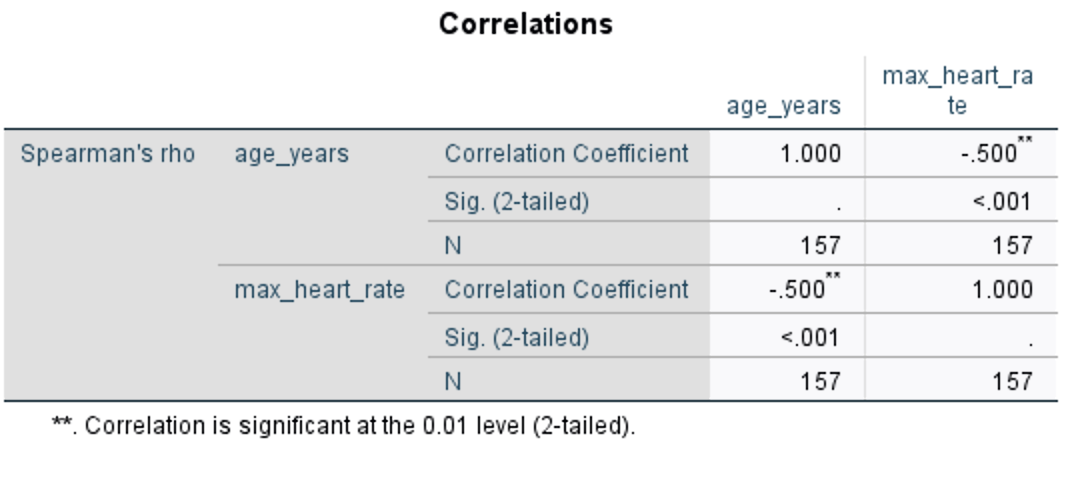
\includegraphics[width=0.65\textwidth]{figures/q3-spearman-result.png}
        \end{center}
        حالا آن را تحلیل می‌کنیم. مقدار
        $p-value$
        کمتر از
        $0.05$
        است پس معنادار است. اما برای بررسی شدت آن باید به سراغ
        \lr{Correlation Coefficient}
        برویم که مقدار
        $-0.5$
        را دارد. با توجه به اینکه
        $|-0.5| = 0.5 > 0.3$
        پس این همبستگی از شدت هم برخوردار است. در واقع ما با یک
        همبستگی معنادار با شدت متوسط روبه رو هستیم که در جهت عکس (مخالف) است.
        بدین معنی که با افزایش سن افراد، حداکثر ضربان قلب آنها کاهش می‌یابد.

        با این حال باید توجه داشته باشیم که این \lr{correlation} رابطه علی و
        \lr{causation} را توجیه نمیکند و صرفا رابطه این دو متغیر را نشان میدهد. چرا که ممکن است عوامل دیگری نیز
        در این رابطه نقش داشته باشند.
    \end{solution}

    \pagebreak

    %%%%%%% AZ 4
    \question سوال ۴:


    \begin{solution}
        ابتدا مقادیر داده شده در صورت سوال را به فرم متعارف مینویسیم:
        \begin{latin}
            \begin{center}
                \begin{tabular}{|c|c|c|}
                    \hline
                                         & \lr{Postive Outcome} & \lr{Negative Outcome} \\
                    \hline
                    \lr{Exposed Group}   & \lr{a}               & \lr{b}                \\
                    \hline
                    \lr{Unexposed Group} & \lr{c}               & \lr{d}                \\
                    \hline
                \end{tabular}
            \end{center}
        \end{latin}

        با توجه به داده‌های صورت سوال داریم:
        \begin{latin}
            \begin{center}
                \begin{tabular}{|c|c|c|}
                    \hline
                                            & \lr{Diseased} & \lr{Non-diseased} \\
                    \hline
                    \lr{Angina Present}     & \lr{69}       & \lr{23}           \\
                    \hline
                    \lr{Angina Not Present} & \lr{56}       & \lr{134}          \\
                    \hline
                \end{tabular}
            \end{center}
        \end{latin}

        برای محاسبه \lr{OR} یا همان \lr{Odds Ratio} از فرمول زیر استفاده میکنیم::
        $$OR = \frac{ad}{bc} = \frac{69 \times 134}{23 \times 56} = 7.179$$
        همچنین برای محاسبه \lr{CI 95\%}
        داریم:
        \begin{align*}
            CI_{95\%} = \exp[\ln(OR) \pm 1.96 \times SE\{\ln(OR)\}]
        \end{align*}
        که مقدار \lr{SE} خود از فرمول زیر به دست می‌اید:
        $$SE\{\ln(OR)\} = \sqrt{\frac{1}{a} + \frac{1}{b} + \frac{1}{c} + \frac{1}{d}}$$
        پس داریم:
        $$SE\{\ln(OR)\} = \sqrt{\frac{1}{69} + \frac{1}{23} + \frac{1}{56} + \frac{1}{134}} = 0.289$$
        و خواهیم داشت:
        $$CI_{95\%} = \exp[\ln(7.179) \pm 1.96 \times 0.289] = [4.074, 12.649]$$


        مقدار \lr{RR} نیز برابر است با:
        $$RR = \frac{a/(a+b)}{c/(c+d)} = \frac{69/(69+23)}{56/(56+134)} = 2.545$$

        حالا به تفسیر جواب‌ها میپردازیم:
        مقدار \lr{OR} برابر با
        \lr{7.179} است. این
        یعنی شانس وجود بیماری عروق کرونر در افراد دارای آنژین ناشی از فعالیت،
        \lr{7.179}
        برابر افراد بدون آنژین است.
        چون فاصله اطمینان شامل عدد
        $1$
        نیست، این ارتباط از نظر آماری معنادار است.

        با توجه به متن سوال، ما با یک مطالعه \lr{Cohort}
        طرف نیستیم و مطالعه با توجه به ثبت همزمان یک مطالعه
        \lr{Cross Sectional}
        محسوب میشود. این باعث میشود که ما \lr{RR} را با احتیاط بیان کنیم.
        یعنی نمیتوانیم با اطمینان بگوییم که چون \lr{RR} ما $2.545$ است، پس
        افراد دارای آنژین،
        \lr{2.545}
        برابر افراد بدون آنژین در معرض خطر ابتلا به بیماری عروق کرونر هستند (ریسک ابتلا در آینده).
    \end{solution}

    \pagebreak
    %%%%% AZ 5
    \question سوال ۵:

    \begin{solution}
        خب. چون در صورت سوال به این موضوع اشاره شده که عرض از مبدأ در نظر گرفته شود،
        در مرحله نخست باید در کنار متغیرهای اولیه دیتاست، یک ستون شامل $1$
        به مجموعه‌ی دیتا اضافه کنیم (همان
        \lr{Intercept}). برای اینکار از قطعه کد زیر  بهره میجوییم:

        \begin{center}
            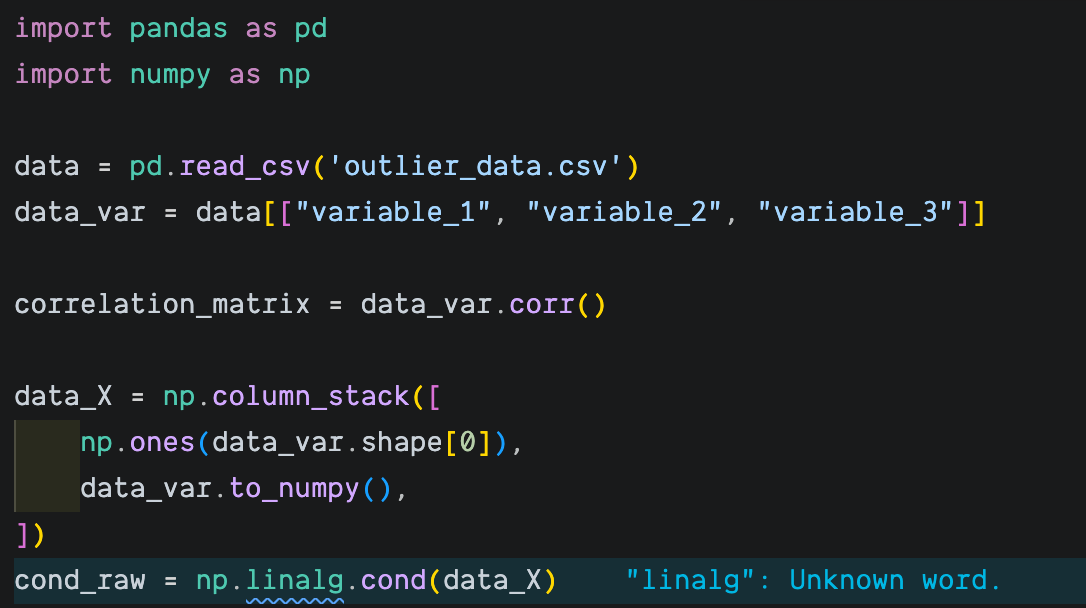
\includegraphics[width=0.65\textwidth]{figures/q5-condition-number-code.png}
        \end{center}

        البته در وهله اول ماتریس همبستگی را هم در متغیری ذخیره کردیم تا بعدا آن را نمایش دهیم.

        در مرحله ی بعدی هم باید استداردسازی را با توجه به فرمول زیر انجام دهیم:
        $$z = \frac{x - mean}{sd}= \frac{x - \mu}{\sigma}$$

        \begin{center}
            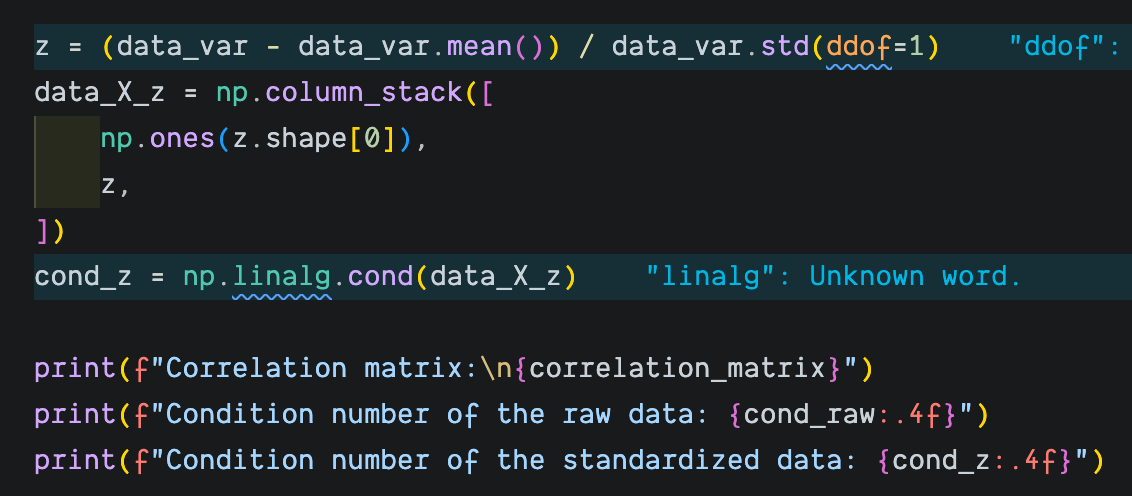
\includegraphics[width=0.65\textwidth]{figures/q5-standardized-code.png}
        \end{center}

        حالا نتایج را در زیر آورده و به بررسی آنها میپردازیم:

        \begin{center}
            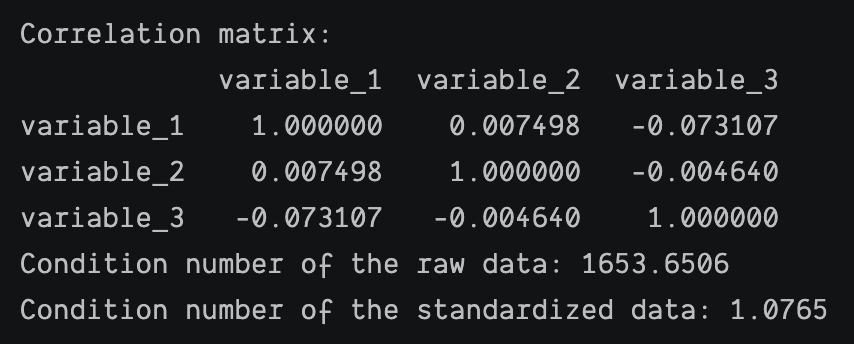
\includegraphics[width=0.65\textwidth]{figures/q5-condition-number-result.png}
        \end{center}
        خب. همانطور که در تصویر مشخص است کاندیشن نامبر دیتای اولیه برابر با
        $1653.650$
        بود. اما پس از استانداردسازی به طرز قابل توجهی به
        $1.077$
        کاهش پیدا کرد.
        از طرفی، وقتی به ماتریس همبستگی آنها نگاه میکنیم به اعداد
        $0.007, -0.073, 0.005$
        برخورد می‌کنیم که تقریبا برابر با صفر هستند. یعنی همبستگی خاصی بین ستون‌ها (ویژگی‌ها) وجود نداشته است.
        همه‌ی اینها باعث میشوند تا نتیجه بگیریم که بالا بودن عدد شرطی قبل از استانداردسازی نه بخاطر همخطی شدید، بلکه به خاطر تفاوت مقایسها رخ داده است.
    \end{solution}

    \pagebreak
    %%%%%% AZ 6
    \question سوال ۶:

    \begin{solution}
        چون
        \lr{outcome\_cad}
        یک متغیر باینری است،
        از منوی
        \lr{Analyze -> Regression -> Binary Logistic}
        وارد شده و طبق تصویر متغیرهای خواسته شده را در قسمت
        \lr{Covariates} قرار میدهیم. سپس در قسمت
        \lr{Categorical} متغیر
        \lr{outcome\_cad} را قرار داده و روی گزینه
        \lr{Categorical}
        میزنیم و چون متغیرهای
        \lr{sex\_male}
        و
        \lr{exercise\_angina\_yes}
        کتگوریکال یا همان کیفی بودند، آن ها را طبق تصویر مشخص و اضافه میکنیم و در نهایت گزینه
        \lr{First}
        را زده و روی
        \lr{Continue}
        کلیک می‌کنیم:

        \begin{center}
            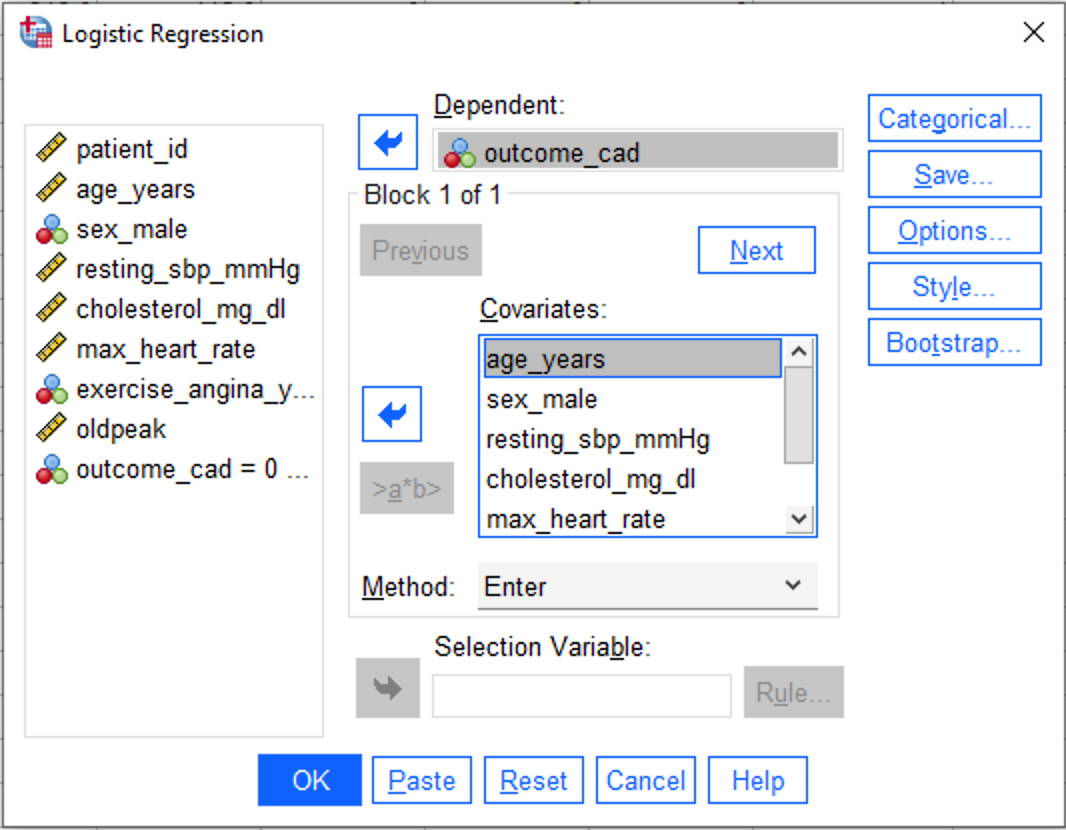
\includegraphics[width=0.5\textwidth]{figures/q6-logistic-regression-dialog.png}
            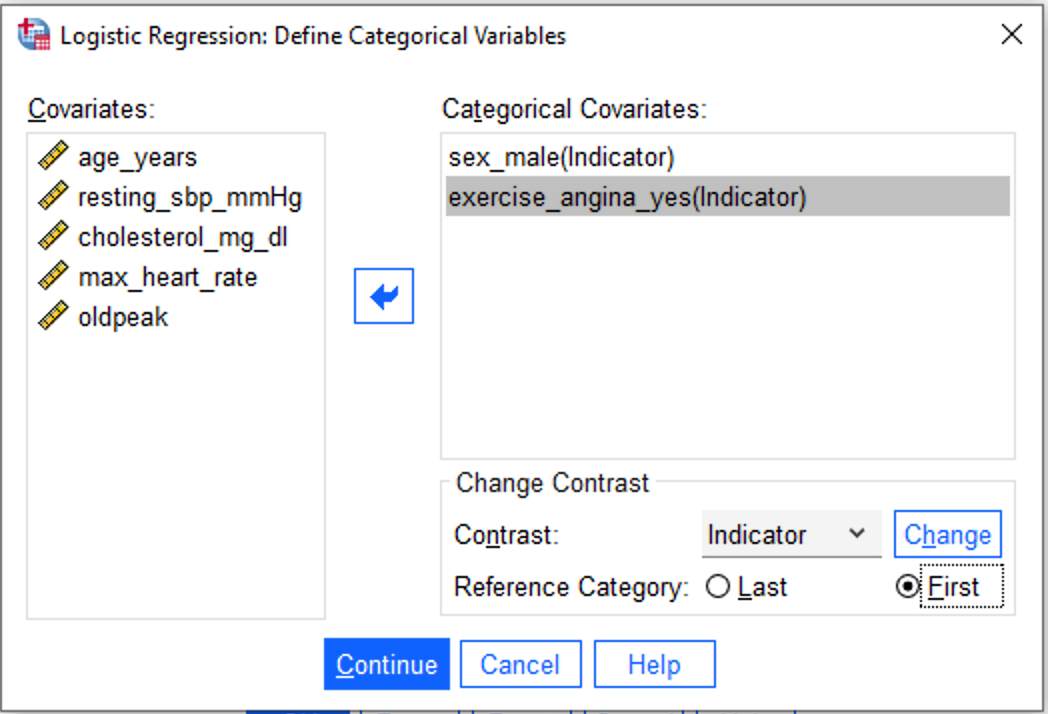
\includegraphics[width=0.50\textwidth]{figures/q6-categorical-covariates.png}
        \end{center}

        سپس در قسمت
        \lr{Options}
        وارد شده و تیک گزینه‌های
        \lr{Hosmer-Lemeshow goodness-of-fit} و \lr{CI 95\%} را زده و روی گزینه
        تایید کلیک می‌کنیم. در واقع این موارد در صورت سوال ذکر شده بودند و نیازشان خواهیم داشت.
        نکته اینجاست که تیک گزینه
        \lr{Include constant}
        را برنمیداریم تا بعد از دیدن \lr{p-value}
        آن تصمیم بگیریم که معنادار است یا خیر:
        \begin{center}
            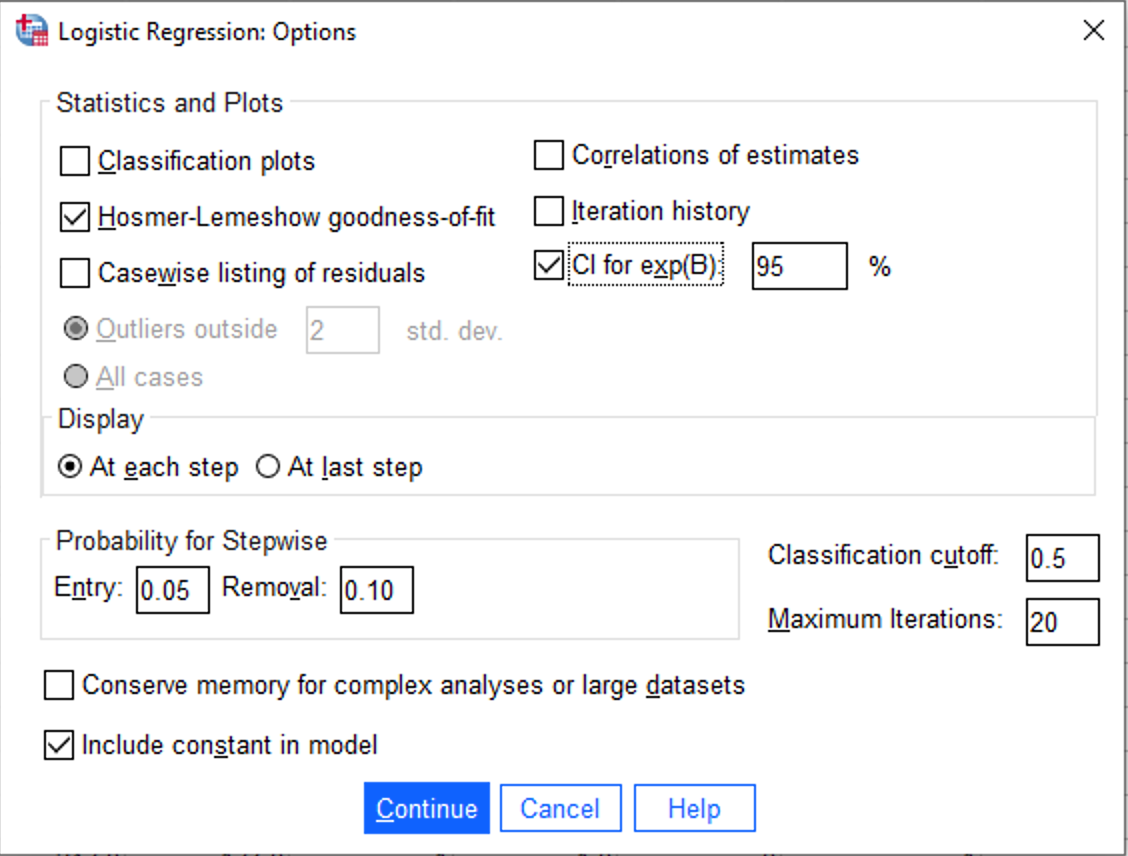
\includegraphics[width=0.65\textwidth]{figures/q6-options.png}
        \end{center}

        در نهایت هم
        در قسمت
        \lr{Save}
        وارد شده و تیک گزینه
        \lr{Probabilities} را میزنیم تا در نتایج مورد نظر ما احتمالات هم وجود داشته باشد:
        \begin{center}
            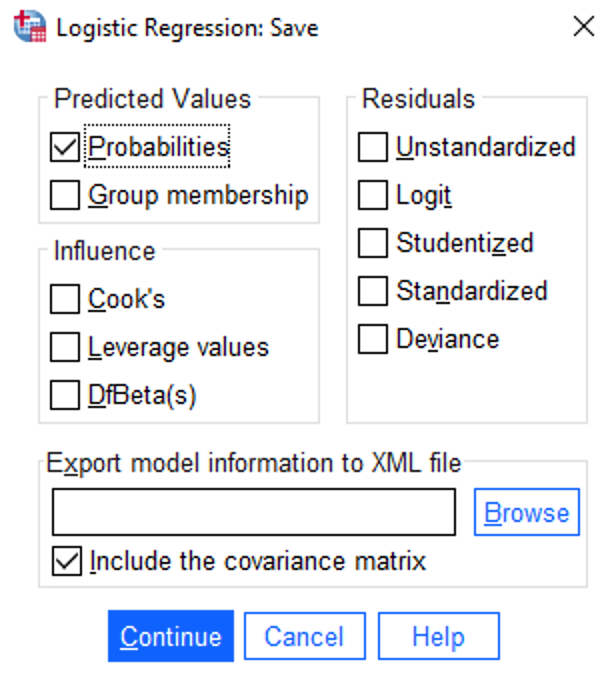
\includegraphics[width=0.65\textwidth]{figures/q6-save.png}
        \end{center}

        حالا با خیال راحت روی گزینه
        \lr{OK}
        میزنیم. نتیجه به صورت زیر است:
        \begin{center}
            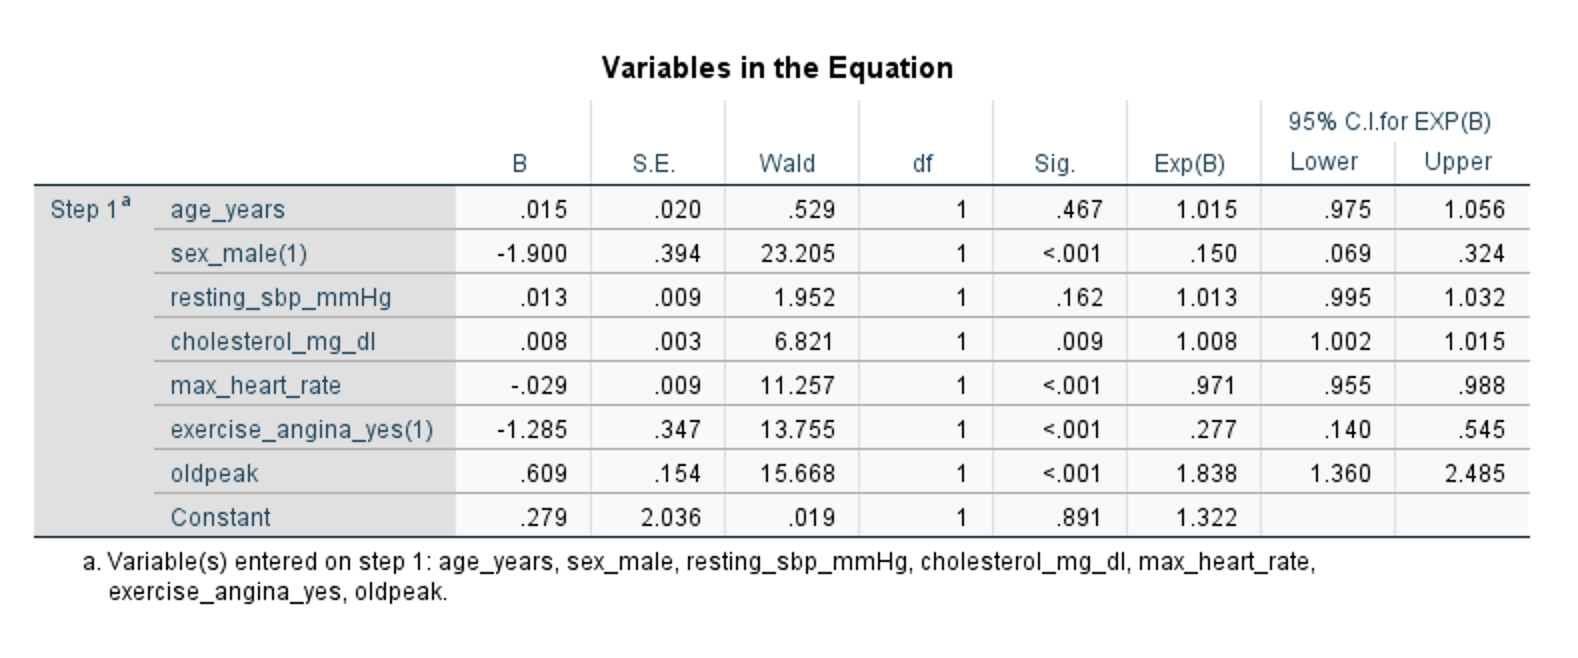
\includegraphics[width=0.65\textwidth]{figures/q6-coefficients.png}
        \end{center}
        همانطور که میبینیم مقدار
        \lr{p-value}
        برای
        \lr{Constant}
        یا همان
        $\beta_0$
        ما به طرز واضحی از $0.05$
        بیشتر است (0.891 > 0.05)
        که نوید از معنادار نبود این ضریب میدهد. به ناچار مدل را دوباره اجرا می‌کنیم ولی این بار دیگر آن تیک مذکور را نمیزنیم:
        \begin{center}
            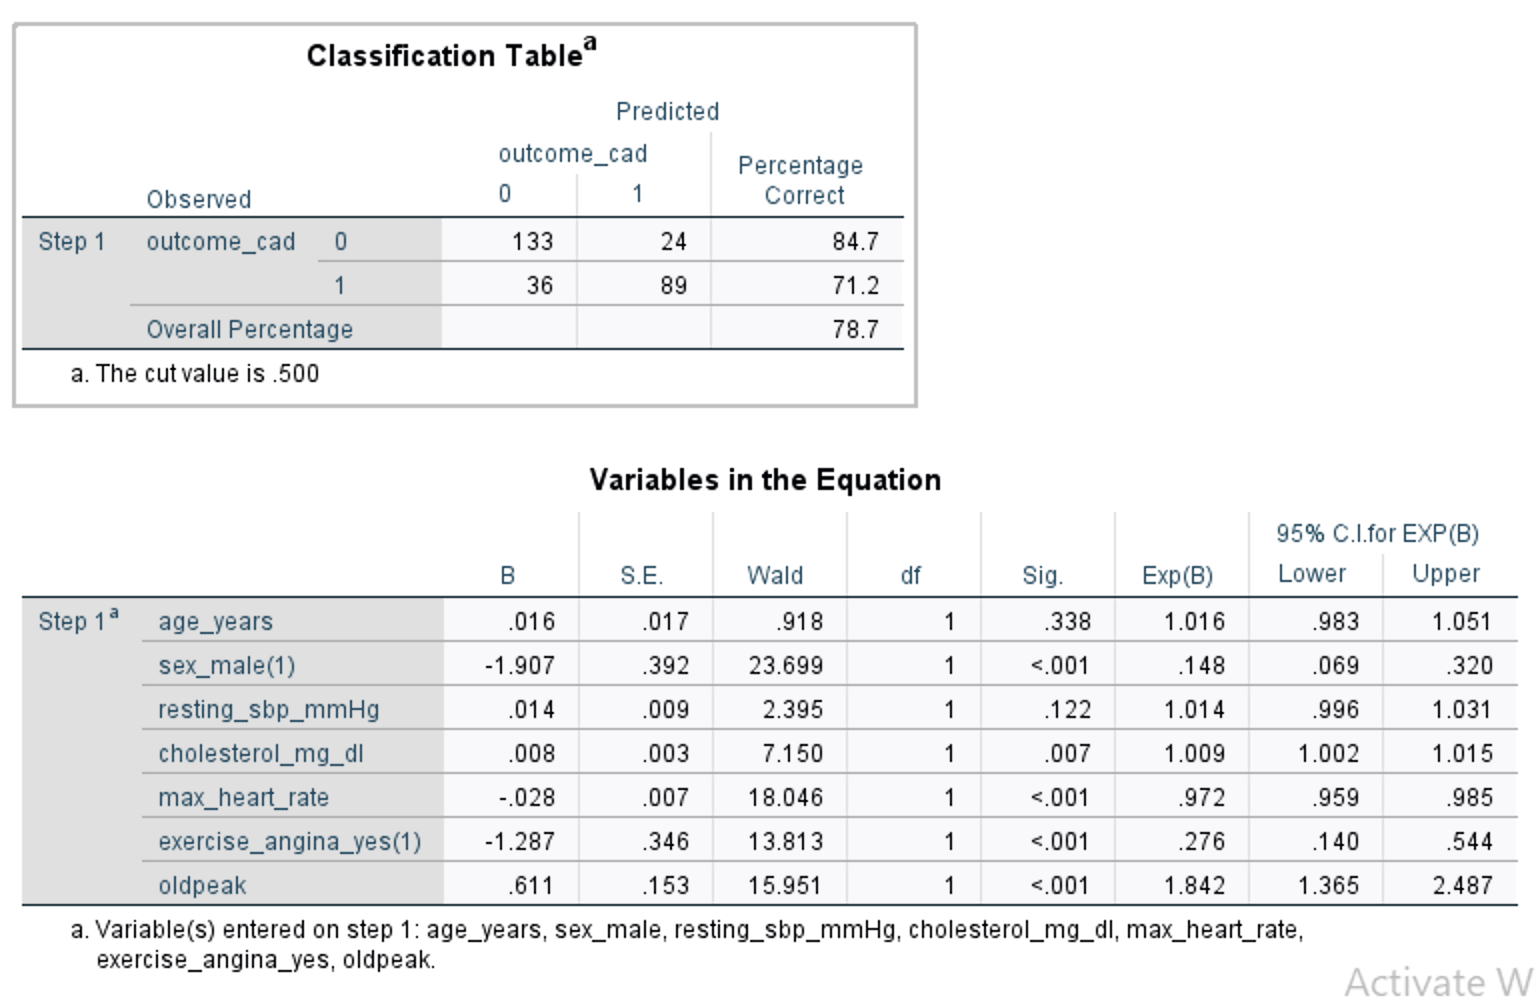
\includegraphics[width=0.65\textwidth]{figures/q6-classification-table.png}
        \end{center}
        با توجه به سطر
        \lr{exercise\_angina\_yes(1)}
        مقدار ضریب آن (ضریب بتا) برابر با
        $-1.287$
        است. چون این ضریب منفی است، نتیجه میگیریم که این فیچر یک
        یک \lr{protective factor} است. یعنی با افزایش این متغیر، احتمال ابتلا به بیماری عروق کرونر کاهش می‌یابد.
        از طرفی میدانیم که مقدار
        $OR = e^{\beta}$
        است پس از روی ستون
        $Exp(B)$
        مقدار آن برابر با
        $0.276$
        خواهد بود. در نتیجه با توجه به اینکه این مقدار کمتر از یک شده است
        میتوان نتیجه گرفت که متبلا نبودن به CAD ارتباط بیشتری با آنژین فعالیت داشتن دارد (یعنی آنژین داشتنش ارتباط بیشتری با CAD نداشتنش دارد).
        در مورد \lr{p-value} هم باید گفت که زیر
        $0.05$ است پس معنادار است و نشان میدهد که این یک فیچر مهم است.
        در ادامه هم با توجه به جدول، $CI_{95\%}$
        را داریم که عبارت است از:
        $$CI_{95\%} = [0.140, 0.544]$$
    \end{solution}

    \pagebreak
    %%%%%% AZ 7
    \question سوال ۷:

    \begin{solution}
        خب. مشخصا در صورت سوال ذکر شده که آستانه را باید روی
        $0.5$
        تنظیم کرد. پس با توجه به کد پایتون زیر اقدام به بررسی فولدهای مختلف میکنیم. دقت کنیم که با استفاده از
        تابع
        \lr{confusion\_matrix}
        استفاده کردیم که به صورت
        \lr{aggregated}
        اقدام به محاسبه چهارمقدار
        $tn$, $fp$, $fn$, $tp$
        خواهد کرد و سپس نتیجه را به صورت کلی اعلام می‌کند:
        \begin{center}
            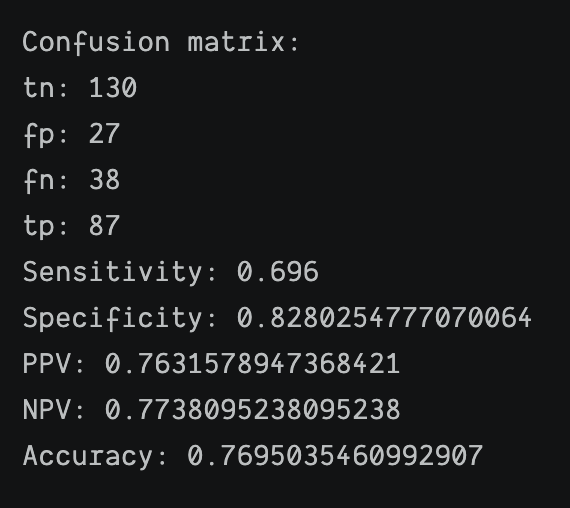
\includegraphics[width=0.37\textwidth]{figures/q7-confusion-matrix-result.png}
            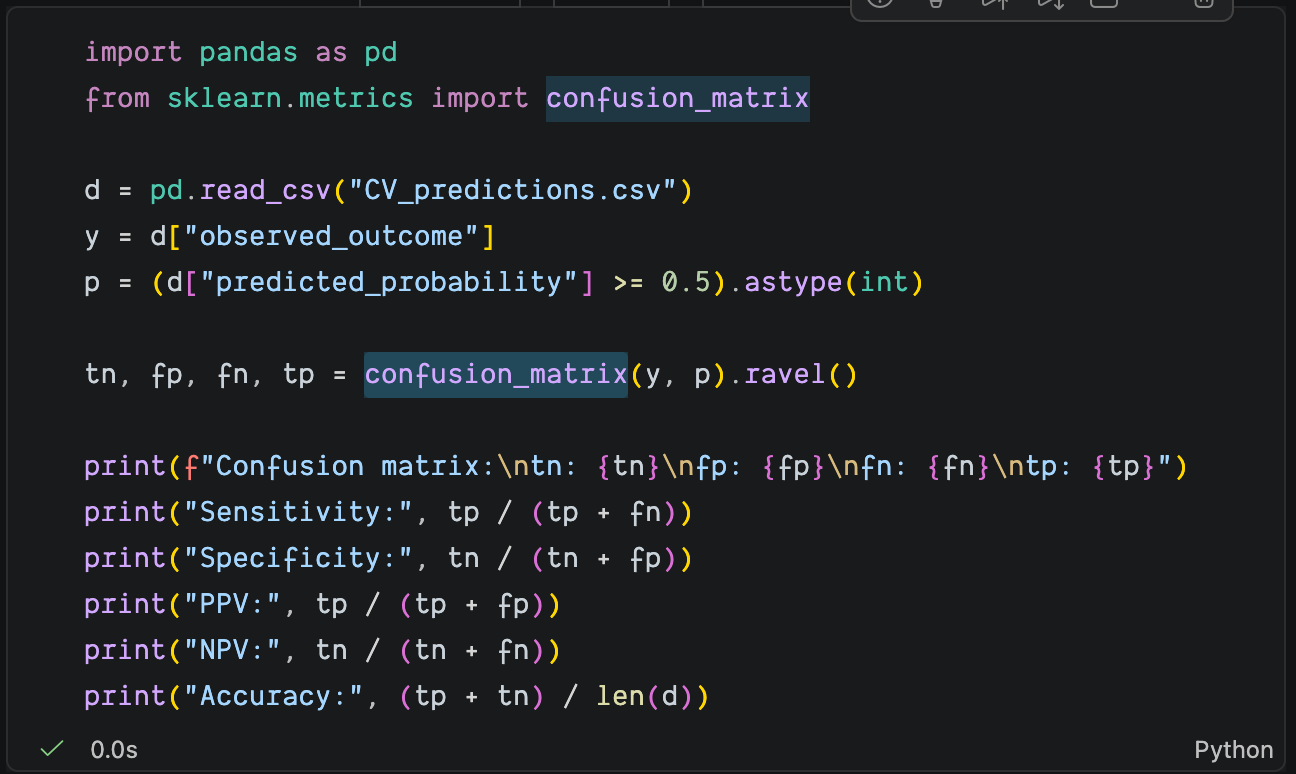
\includegraphics[width=0.55\textwidth]{figures/q7-confusion-matrix-code.png}
        \end{center}

        طبق تصویر داریم:
        \begin{align*}
            Se  & = 69.6\%   \\
            Sp  & = 82.803\% \\
            PPV & = 76.316\% \\
            NPV & = 77.381\% \\
            Acc & = 76.950\%
        \end{align*}

        و این یعنی اینکه:
        \begin{itemize}
            \item مقدار Se به ما نشان میدهد که مدل تقریبا
                  در ۷۰ درصد مواقع، موارد مثبت را به درستی تشخیص می‌دهد.
            \item از طرفی Sp هم نشان میدهد که مدل تقریبا در ۸۳ درصد مواقع،
                  موارد منفی را به طور صحیح تشخیص می‌دهد.
            \item مقدار PPV به این معنی است که تقریبا در ۷۶ درصد مواقع، مواردی که مثبت تشخیص داده شده بودند واقعا هم مثبت بودند.
            \item سپس NPV میگوید که تقریبا در ۷۷ درصد مواقع مواردی که منفی تشخیص داده شده‌اند، واقعا منفی بوده‌اند.
            \item در نهایت Acc ۷۷ درصدی نیز بدین معنی است که تقربیا در ۷۷ درصد مواقع یک طبقه‌بندی درست به ما می‌دهد.
        \end{itemize}
        تفسیر ما میتواند این باشد که مدل در شناسایی افراد واقعاً منفی، با ویژگی
        $82\..8\%$
        ،بهتر از یافتن همهٔ موارد
        ابتلا با حساسیت
        $69\..6\%$
        عمل می‌کند.

        البته ما این کار را بدون aggregation همی میشد انجام دهیم. یعنی به ازای هر فولد
        مقادیر را محاسبه کنیم و پاسخ را به اپ مورد اشاره در صورت سوال بدهیم. در این صورت با کد زیر به
        نتیجه زیر میرسیدیم:
        \begin{center}
            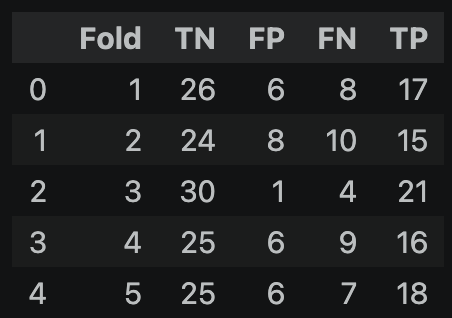
\includegraphics[width=0.33\textwidth]{figures/q7-per-fold-result.png}
            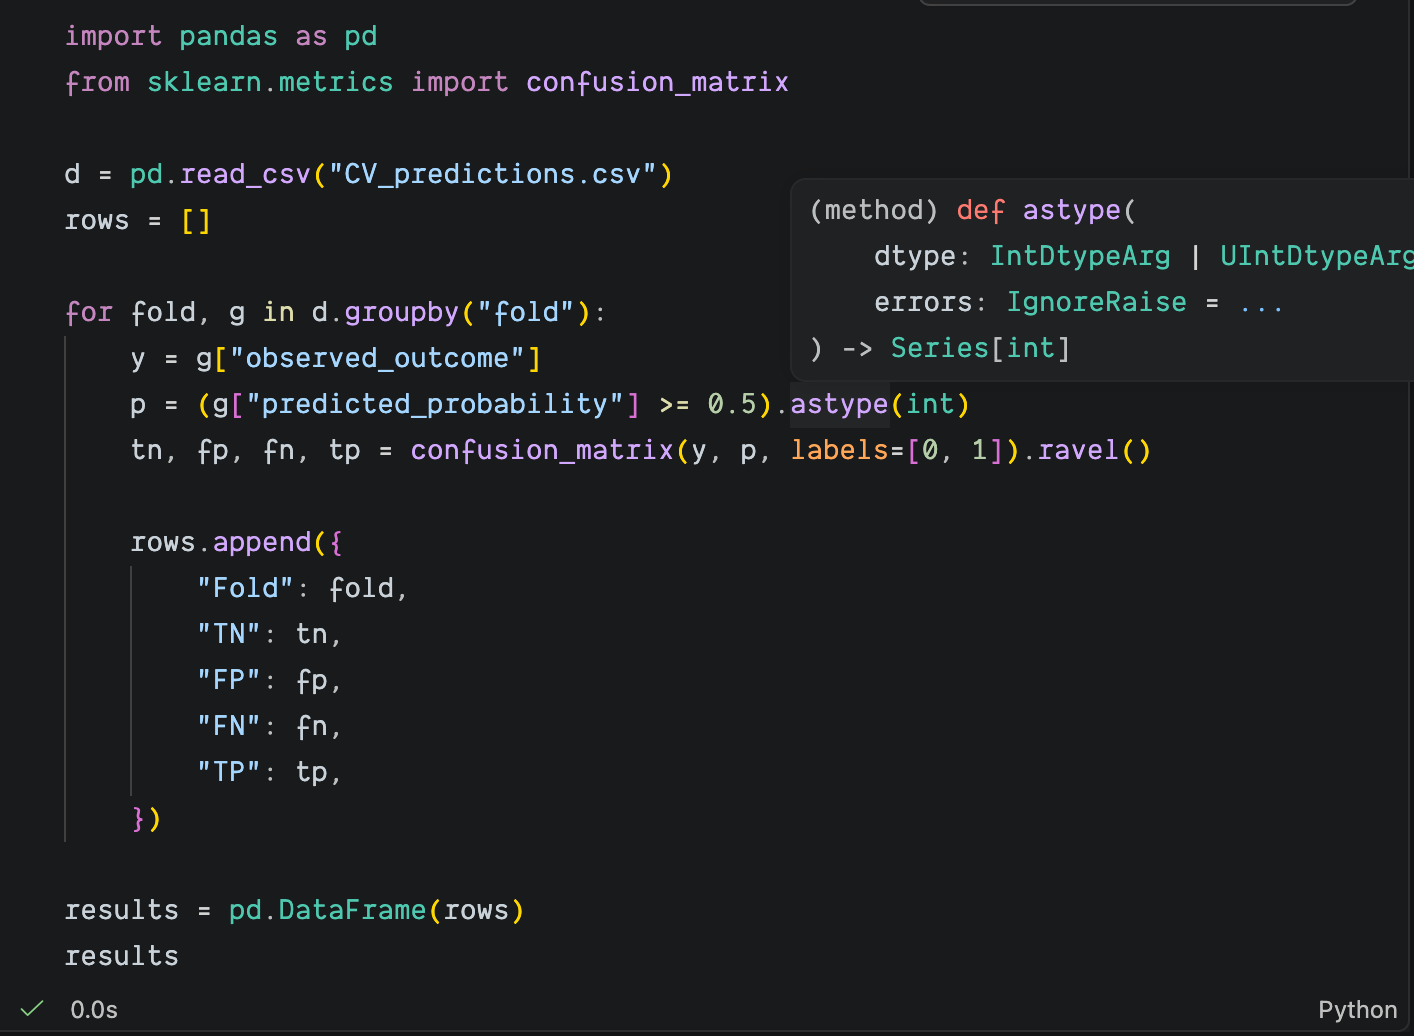
\includegraphics[width=0.33\textwidth]{figures/q7-per-fold-code.png}
        \end{center}
        سپس با دادن مقادیر به اپ، نتیجه زیر را میداشتیم:
        \begin{center}
            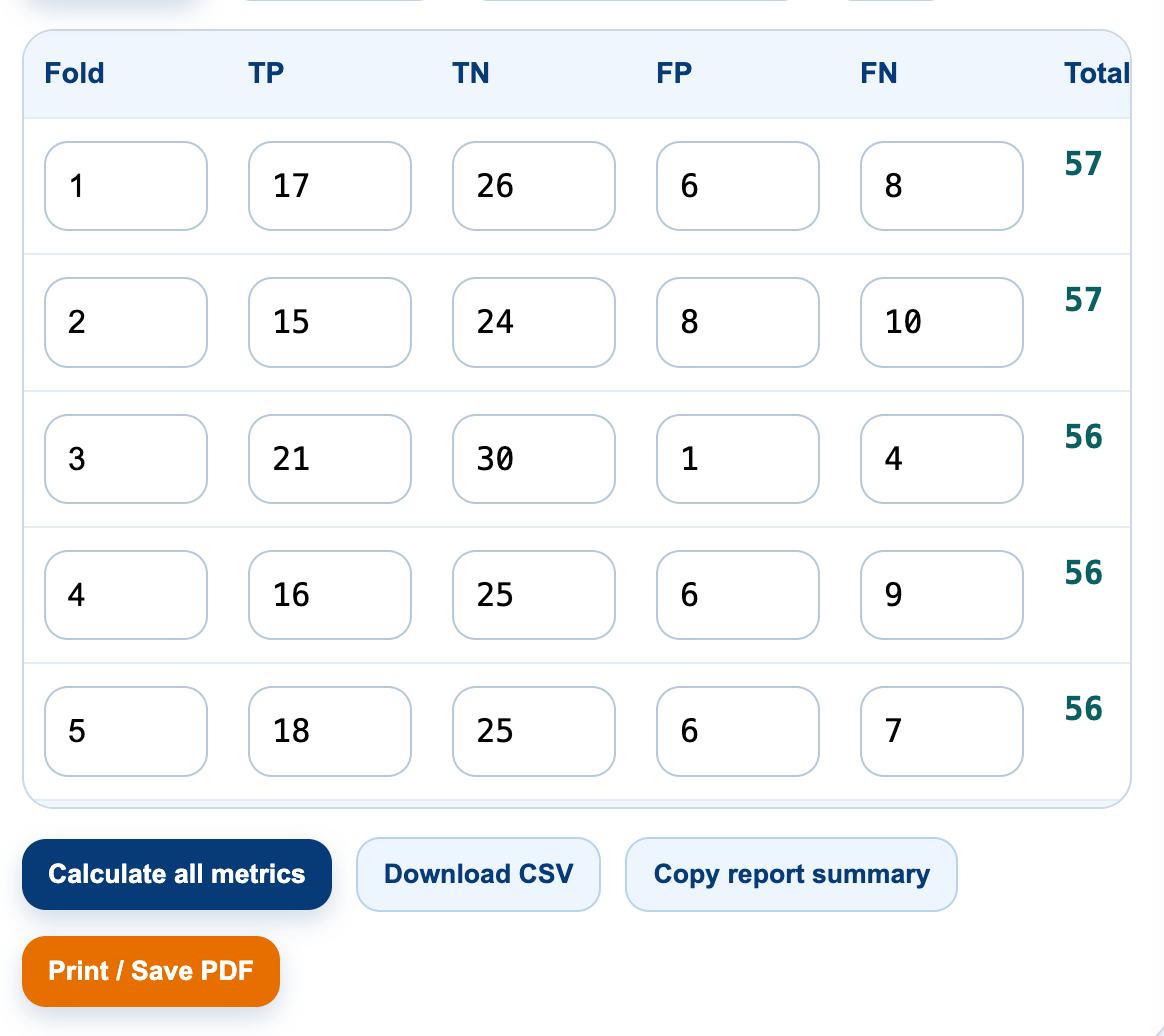
\includegraphics[width=0.50\textwidth]{figures/q7-calculator-folds.png}
            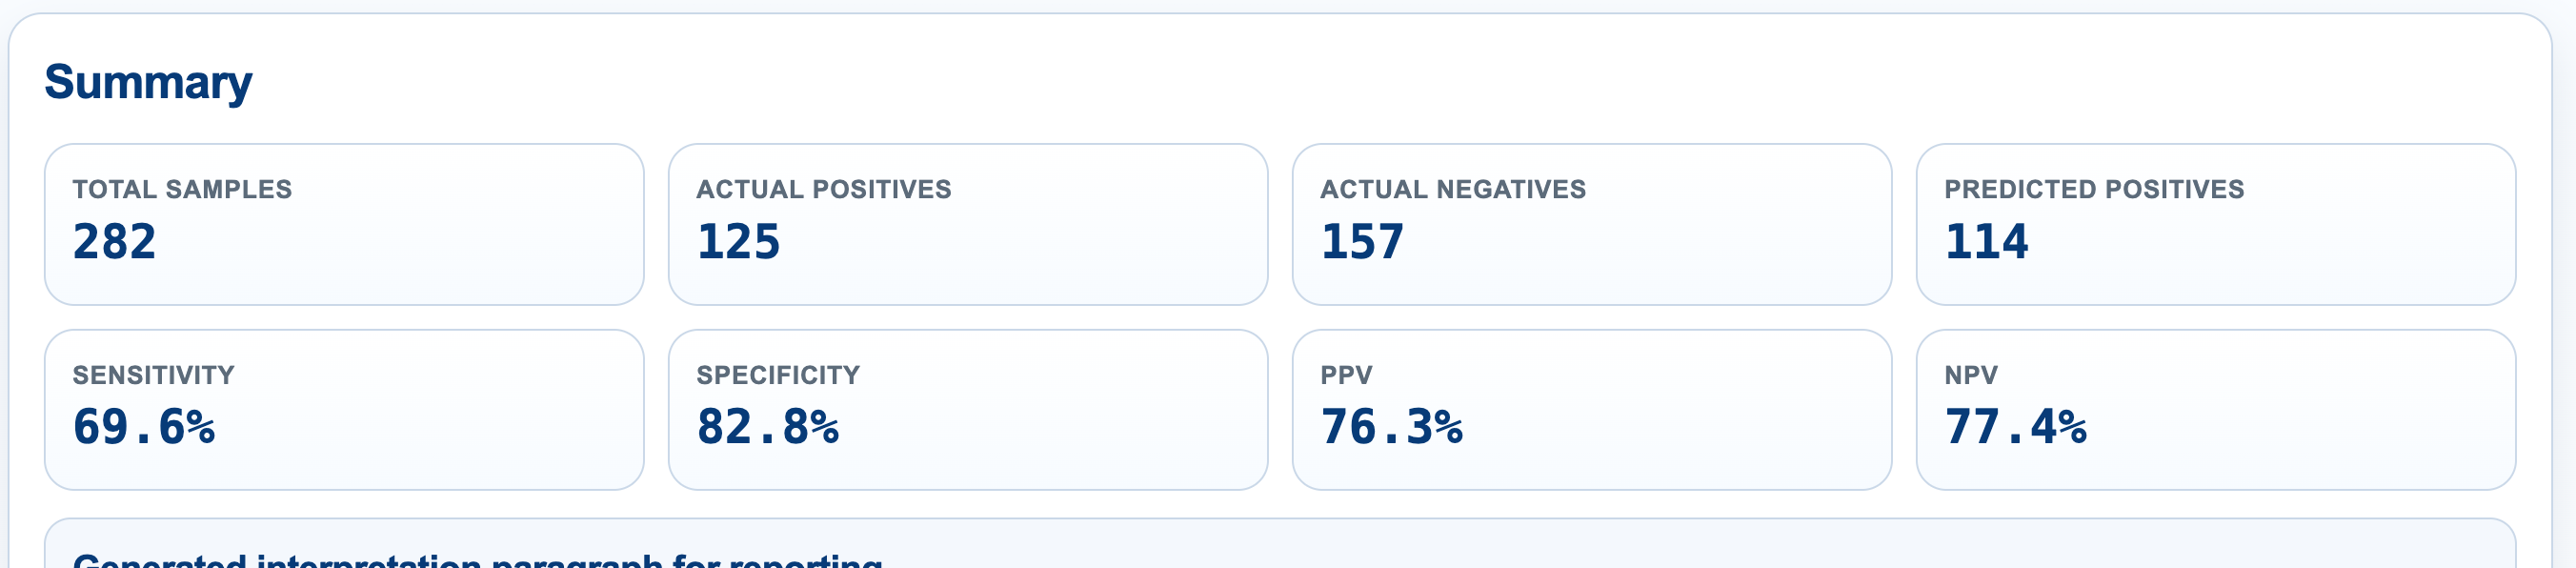
\includegraphics[width=0.65\textwidth]{figures/q7-calculator-summary.png}
            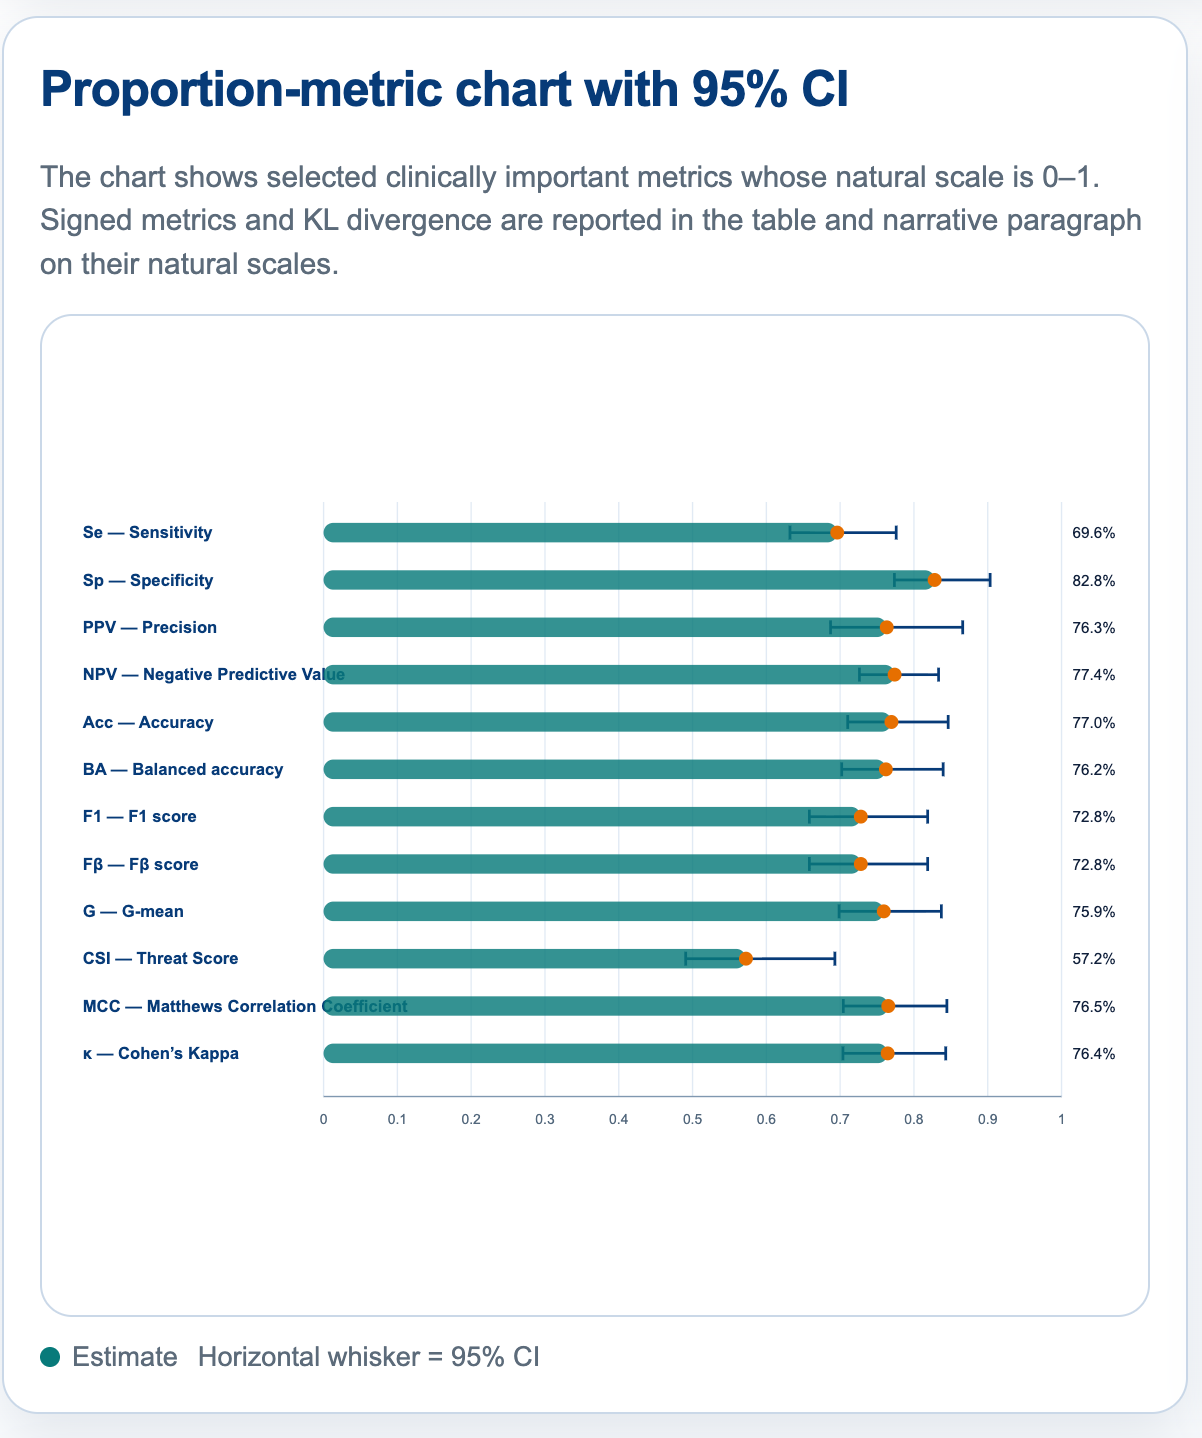
\includegraphics[width=0.53\textwidth]{figures/q7-metrics-chart.png}
        \end{center}
        که مشاهده می‌شود نتایج آن مطابق با نتایج متد قبلی است.

    \end{solution}

    \pagebreak

    \question سوال ۸:
    \begin{solution}

        \textbf{الف:}

        همان کد قبلی را اجرا می‌کنیم ولی به جای
        $0.5$
        از
        $0.3$
        استفاده می‌کنیم. نتیجه به صورت زیر خواهد بود:
        \begin{center}
            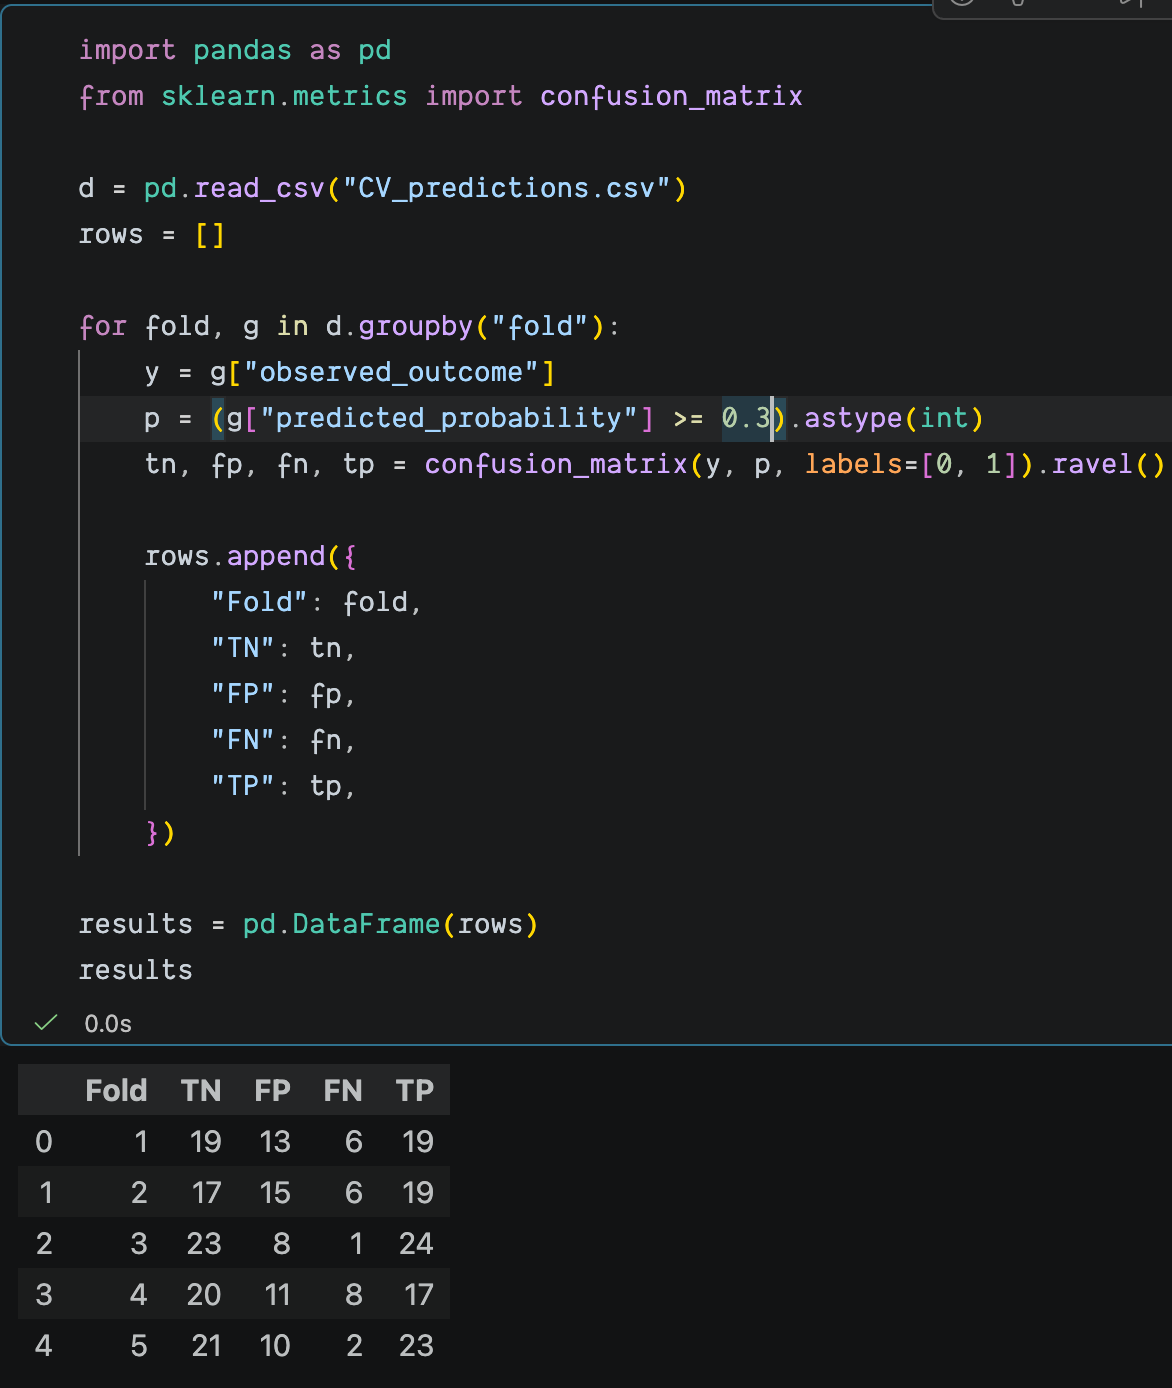
\includegraphics[width=0.45\textwidth]{figures/q8-per-fold.png}
            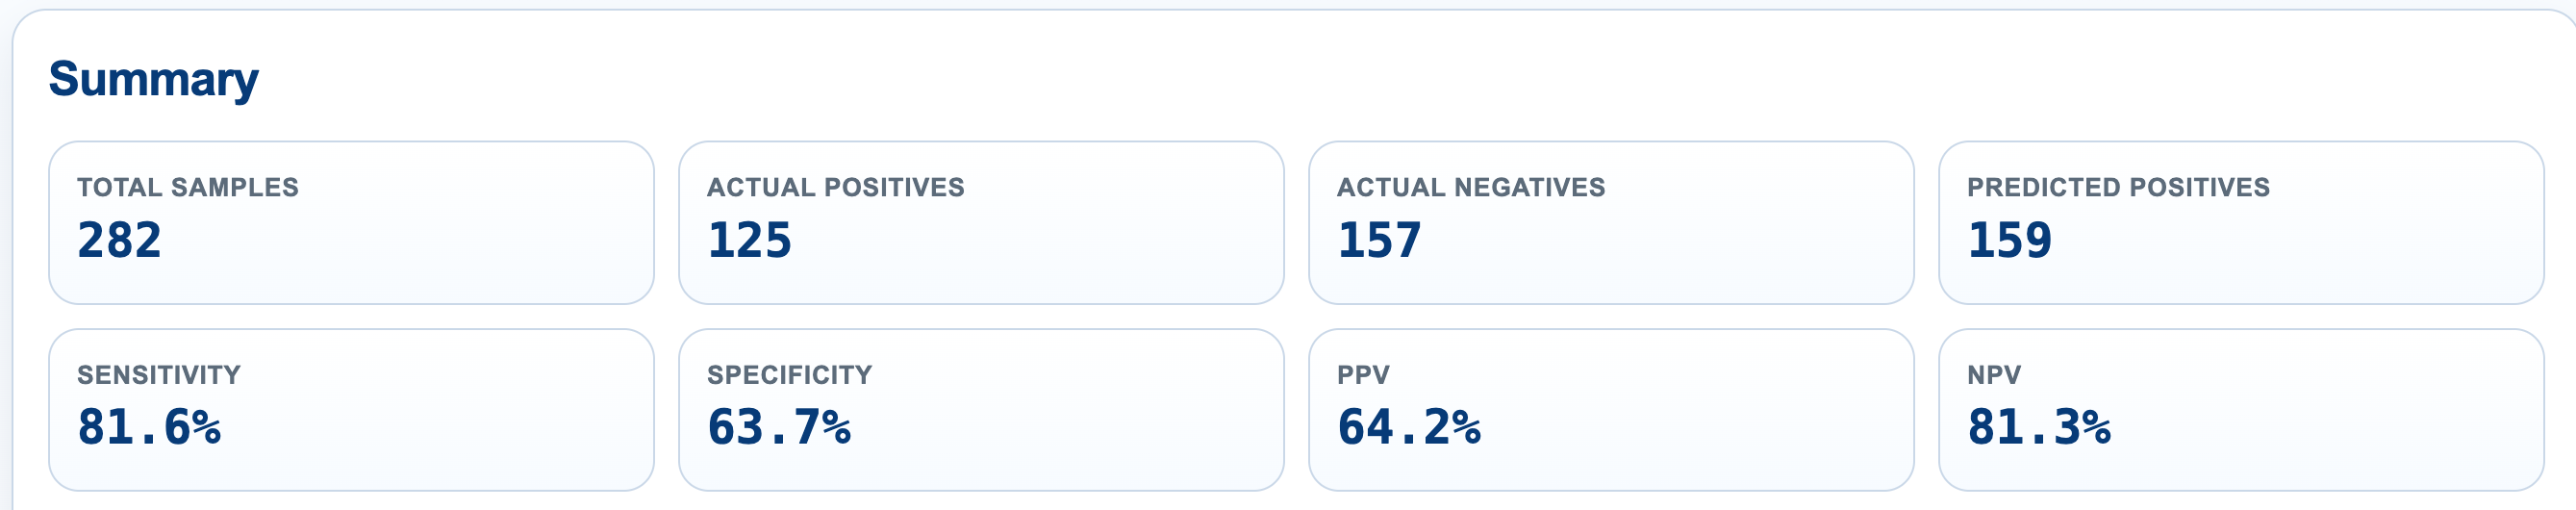
\includegraphics[width=0.65\textwidth]{figures/q8-calculator-summary.png}
            
\includegraphics[width=0.65\textwidth]{figures/q8-accuracy-interval.png}
        \end{center}
        که عبارتند از:
        \begin{align*}
            Se  & = 81.6\% \\
            Sp  & = 63.7\% \\
            PPV & = 64.2\% \\
            NPV & = 81.3\% \\
            Acc & = 71.6\%
        \end{align*}

        همانطور که مشخص است وقتی این موارد را با موارد سوال قبلی که با $0.5$
        به دست آورده شده بودند مقایسه میکنیم، متوجه افزایش $Se$ میشویم. این بدان معنی است
        مدل در مشخص کردن موارد مثبت بهتر عمل می‌کند. اما این تغییر آستانه با کاهش
        ویژگی یا همان $Sp$ هم همراه بوده. پس برای
        پاسخ به قسمت الف باید گفت آن وقتهایی که برای ما تشخیص مثبت بودن بیماری اهمیت بیشتری دارد این آستانه بهتر است. در غیر این صورت همان آستانه قبلی مناسب‌تر است.

        \textbf{ب:}
        با توجه به صورت سوال تابع هزین هرا به صورت زیر مینویسیم:
        $$Cost(t) = 4FN_t + FP_t$$
        با توجه به جداولی که در این سوال و سوال قبل داشتیم، برای آستانه
        $0.5$
        داشتیم $FN = 38$ و $FP = 27$ پس تابع میشود:
        $$Cost(0.5) = 4(38) + 27 = 152 + 27 = 179$$
        همینطور برای $0.3$ داشتیم
        $FN = 23$ و $FP = 57$ پس تابع میشود:
        $$Cost(0.3) = 4(23) + 57 = 92 + 57 = 149$$
        چون هزینه در آستانه $0.3$ کمتر شد، آن را برای غربالگری انتخاب میکنیم. با توجه به
        فرمول،‌ در این تابع هزینه برای ما $FN$ اهمیت بالاتری داشت، یعنی نمیخواستیم کسی که بیمار است را به اشتباه سالم تشخیص دهیم.

        و خب برای بررسی اثر شیوع هم باید این نکته را در نظر داشته باشیم که بر اساس فرمول
        $$PPV = \frac{Se \times Prev}{(Se \times Prev) + ((1 - Sp) \times (1 - Prev))}$$
        شیوع با PPV ارتباط کاملا مستقیمی دارد و با افزایش آن، ما شاهد این خواهیم بود که
        احتمال اینکه نمونه‌های مثبتی که اعلام کردیم واقعا مثبت باشند افزایش پیدا میکند.
    \end{solution}


    \question سوال ۹:
    \begin{solution}
        خب. در این روش دو نوع نشت داده داریم. اول اینکه پژوهشگر محترم قبل از شروع اعتبارسنجی متقاطع، کل دیتا را استاندارد کرده اند. یعنی میانگین و انحراف معیار با استفاده از همهٔ نمونه ها، حتی نمونه‌هایی که بعدا در fold
        \underbar{آزمون}
        قرار می‌گیرند، حساب شده است. پس مدل موقع آموزش به شکل غیرمستقیم از دیتای آزمون هم اطلاعات گرفته است.

        مشکل دومی هم است. بهترین \lr{feature} ها را با استفاده از \lr{outcome\_cad} روی کل دیتا انتخاب کرده‌اند. در این حالت برچسب نمونه‌های آزمون هم در انتخاب \lr{feature} ها دخالت دارد؛ پس دیگر fold آزمون واقعا دیده‌نشده و مستقل نیست.

        برای حل این مشکل باید از \lr{Nested Cross-Validation} استفاده کنیم. مثلا ابتدا دیتا را به پنج fold بیرونی تقسیم می‌کنیم. در هر مرحله یک fold را فقط برای تست نهایی کنار می‌گذاریم و چهار fold دیگر دیتای آموزش ما هستند. این fold آزمون بیرونی نباید در استانداردسازی، انتخاب \lr{feature}، انتخاب مدل یا تنظیم \lr{hyperparameter}ها استفاده شود.

        حالا فقط روی همان چهار fold آموزشی، یک \lr{CV} داخلی اجرا می‌کنیم. در هر تقسیم داخلی، میانگین و انحراف معیار را فقط از بخش train داخلی به دست می‌آوریم و با همان مقادیر بخش validation را استاندارد می‌کنیم. انتخاب feature هم باید فقط با استفاده از \lr{outcome\_cad} بخش train داخلی انجام شود. بعد مدل‌ها و تنظیمات مختلف را روی validation داخلی مقایسه کرده و بهترین pipeline را انتخاب می‌کنیم.

        در نهایت بهترین pipeline را از اول روی تمام چهار fold آموزشی بیرونی fit می‌کنیم و فقط یک بار روی fold آزمون بیرونی پیشبینی می‌گیریم. این کار را برای همهٔ foldهای بیرونی تکرار کرده و در آخر پیشبینی‌ها را با هم تجمیع میکنیم تا \lr{AUROC} را به دست آوریم.

        به این شکل، هر فرد با مدلی پیش‌بینی می‌شود که آن فرد نه در fit مدل و نه در انتخاب featureها و تنظیمات آن حضور نداشته است. پس \lr{AUROC} به دست آمده واقعی تر است. در حالت نشت داده معمولا \lr{AUROC} به شکل خوش‌بینانه بیشتر از عملکرد واقعی مدل گزارش می‌شود؛ مخصوصا وقتی انتخاب feature با استفاده از کل \lr{outcome} انجام شده باشد.
    \end{solution}

    \question سوال ۱۰:
    \begin{solution}
        چون مقدار \lr{AUROC} هر دو مدل برابر با $0.83$ است. پس از نظر قدرت تفکیک تفاوتی با هم ندارند؛ یعنی هر دو مدل تقریبا به یک اندازه می‌توانند افراد پرخطر را از افراد کم‌خطر تفکیک کنند.
        بنابراین فقط با نگاه کردن به \lr{AUROC} نمیتوانییم بگوییم کدام مدل بهتر است.

        اما اگر بخواهیم احتمال خطر را پیش‌بینی کنیم، مدل \lr{A} انتخاب بهتری است. مقدار مورد نظر ما برای شیب کالیبراسیون $1$ و برای عرض از مبدا $0$ است. در مدل \lr{A} این دو مقدار به ترتیب $0.98$ و $0.02$ هستند که خیلی به مقادیر ایده‌آل نزدیک‌اند. پس احتمال‌هایی که این مدل می‌دهد قابل اعتمادتر هستند.

        اختلاف مقدار شبه $R^2$ برای دو مدل $0.02$ است که تفاوت خاصی ایجاد نمیکند
        و دو مدل می‌توانند \lr{AUROC} یکسانی داشته باشند ولی احتمال‌های خیلی متفاوتی تولید کنند.

        برای اینکه کالیبراسیون مدل را بهتر بررسی کنیم، می‌توانیم نمودار کالیبراسیون رسم کنیم. در این نمودار احتمال پیش‌بینی‌شده را با فراوانی واقعی پیامد مقایسه می‌کنیم. اگر نقاط روی خط $45$ درجه باشند، یعنی کالیبراسیون مدل خوب است. این نمودار علاوه بر شیب و عرض از مبدا، نشان می‌دهد که آیا در بعضی نواحی مدل خطر را بیش‌برآورد یا کم‌برآورد کرده است یا نه. با توجه به شیب $0.98$ و عرض از مبدا $0.02$، انتظار داریم منحنی کالیبراسیون مدل \lr{A} به خط ایده‌آل نزدیک‌تر باشد؛ پس باز هم مدل \lr{A} را ترجیح می‌دهیم.
    \end{solution}

\end{questions}
\end{document}
